%%%%%%%%%%%%%%%%%%%%%%%%%%%%%%%%%%%%%%%%%
% Beamer Presentation
% LaTeX Template
% Version 1.0 (10/11/12)
%
% This template has been downloaded from:
% http://www.LaTeXTemplates.com
%
% License:
% CC BY-NC-SA 3.0 (http://creativecommons.org/licenses/by-nc-sa/3.0/)
%
%%%%%%%%%%%%%%%%%%%%%%%%%%%%%%%%%%%%%%%%%

%----------------------------------------------------------------------------------------
%	PACKAGES AND THEMES
%----------------------------------------------------------------------------------------

\documentclass{beamer}

\mode<presentation> {

% The Beamer class comes with a number of default slide themes
% which change the colors and layouts of slides. Below this is a list
% of all the themes, uncomment each in turn to see what they look like.

%\usetheme{default}
%\usetheme{AnnArbor}
%\usetheme{Antibes}
%\usetheme{Bergen}
%\usetheme{Berkeley}
%\usetheme{Berlin}
%\usetheme{Boadilla}
%\usetheme{CambridgeUS}
%\usetheme{Copenhagen}
%\usetheme{Darmstadt}
%\usetheme{Dresden}
%\usetheme{Frankfurt}
%\usetheme{Goettingen}
%\usetheme{Hannover}
%\usetheme{Ilmenau}
%\usetheme{JuanLesPins}
%\usetheme{Luebeck}
\usetheme{Madrid}
%\usetheme{Malmoe}
%\usetheme{Marburg}
%\usetheme{Montpellier}
%\usetheme{PaloAlto}
%\usetheme{Pittsburgh}
%\usetheme{Rochester}
%\usetheme{Singapore}
%\usetheme{Szeged}
%\usetheme{Warsaw}

% As well as themes, the Beamer class has a number of color themes
% for any slide theme. Uncomment each of these in turn to see how it
% changes the colors of your current slide theme.

%\usecolortheme{albatross}
%\usecolortheme{beaver}
%\usecolortheme{beetle}
%\usecolortheme{crane}
%\usecolortheme{dolphin}
%\usecolortheme{dove}
%\usecolortheme{fly}
%\usecolortheme{lily}
%\usecolortheme{orchid}
%\usecolortheme{rose}
%\usecolortheme{seagull}
%\usecolortheme{seahorse}
%\usecolortheme{whale}
%\usecolortheme{wolverine}

%\setbeamertemplate{footline} % To remove the footer line in all slides uncomment this line
%\setbeamertemplate{footline}[page number] % To replace the footer line in all slides with a simple slide count uncomment this line

%\setbeamertemplate{navigation symbols}{} % To remove the navigation symbols from the bottom of all slides uncomment this line
}

\usepackage{graphicx} % Allows including images
\usepackage{booktabs} % Allows the use of \toprule, \midrule and \bottomrule in tables
\usepackage[utf8]{inputenc}
\usepackage[english,brazil]{babel}
\usepackage{epstopdf}
\usepackage{tikz}
\usepackage{subcaption}
\newcommand\m[1]{\begin{bmatrix}#1\end{bmatrix}} 

%----------------------------------------------------------------------------------------
%	TITLE PAGE
%----------------------------------------------------------------------------------------

\title[]{Controle de um Manipulador Robótico 4-DOF com Software baseado em ROS e Qt} % The short title appears at the bottom of every slide, the full title is only on the title page

\author{Luís Gustavo Oliveira Silva} % Your name

\institute[UFRJ] % Your institution as it will appear on the bottom of every slide, may be shorthand to save space
{
\large{Orientador: Fernando Cesar Lizarralde} \\
\medskip
Universidade Federeal do Rio de Janeiro \\ % Your institution for the title page
\textit{} % Your email address
}
\date{\today} % Date, can be changed to a custom date

\begin{document}

\begin{frame}
\titlepage % Print the title page as the first slide
\end{frame}

%\begin{frame}
%\frametitle{Overview} % Table of contents slide, comment this block out to remove it
%\tableofcontents % Throughout your presentation, if you choose to use \section{} and \subsection{} commands, these will automatically be printed on this slide as an overview of your presentation
%\end{frame}

%----------------------------------------------------------------------------------------
%	PRESENTATION SLIDES
%----------------------------------------------------------------------------------------

%------------------------------------------------
\section{First Section} % Sections can be created in order to organize your presentation into discrete blocks, all sections and subsections are automatically printed in the table of contents as an overview of the talk
%------------------------------------------------

\subsection{Subsection Example} % A subsection can be created just before a set of slides with a common theme to further break down your presentation into chunks

\begin{frame}
\frametitle{Introdução}
Robótica em instalações offshore de óleo e gás.
\begin{itemize}
\item Substituir o uso de diversos sensores.
\item Tarefas repetitivas.
\item Tarefas onde a presença humana é difícil, ou arriscada.
\item Tarefas que requerem interação complexa e precisa com o ambiente.
\end{itemize}

\newlength{\twosubht}
\newsavebox{\twosubbox}

\begin{figure}[htp]
% preliminary
\sbox\twosubbox{%
  \resizebox{\dimexpr.9\textwidth-1em}{!}{%
    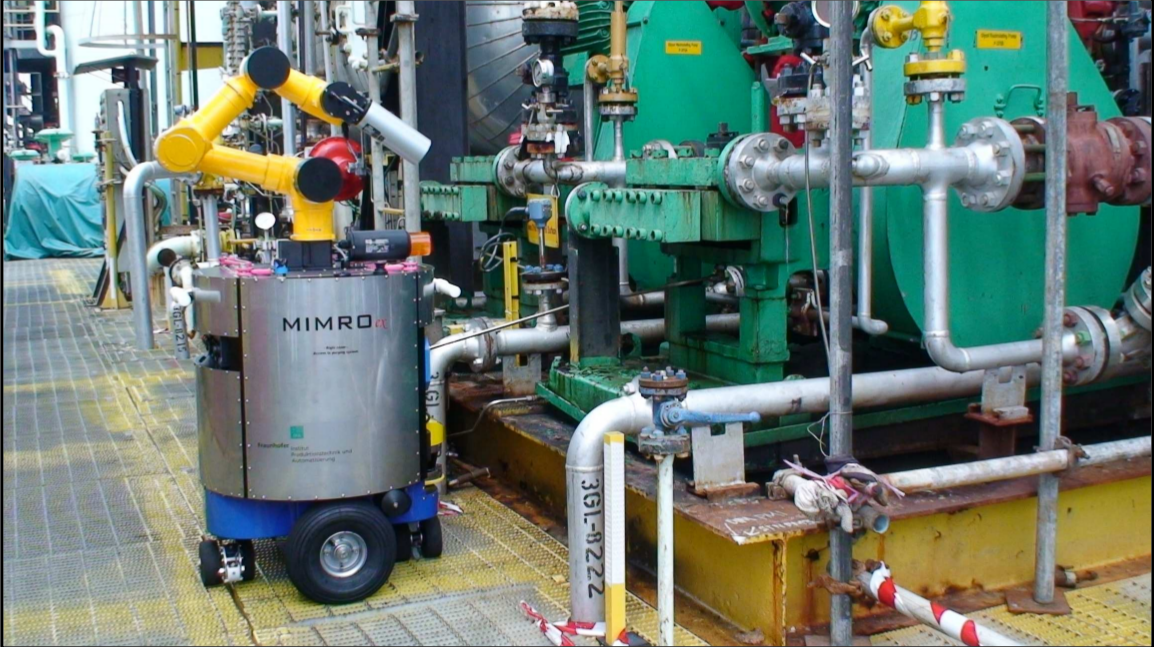
\includegraphics[height=3cm]{./img/mimro.png}%
    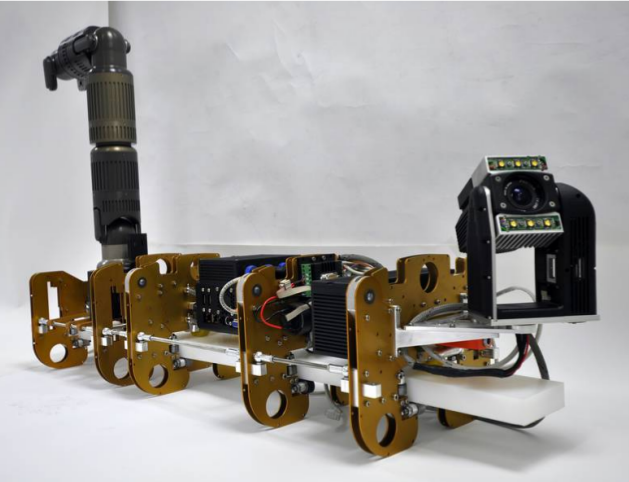
\includegraphics[height=3cm]{./img/artis.png}%
  }%
}
\setlength{\twosubht}{\ht\twosubbox}
% typeset
\centering
\subcaptionbox{MIMROex\label{fig:harmonic_drive}}{%
  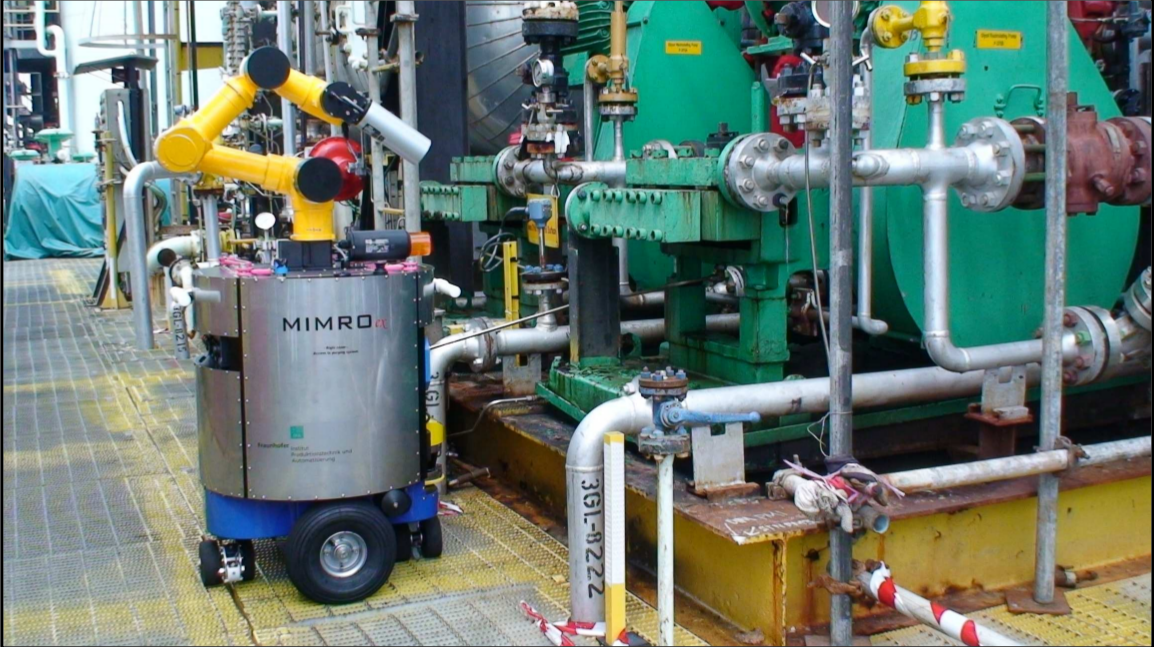
\includegraphics[height=\twosubht]{./img/mimro.png}%
}\quad
\subcaptionbox{ARTIS\label{fig:epos}}{%
  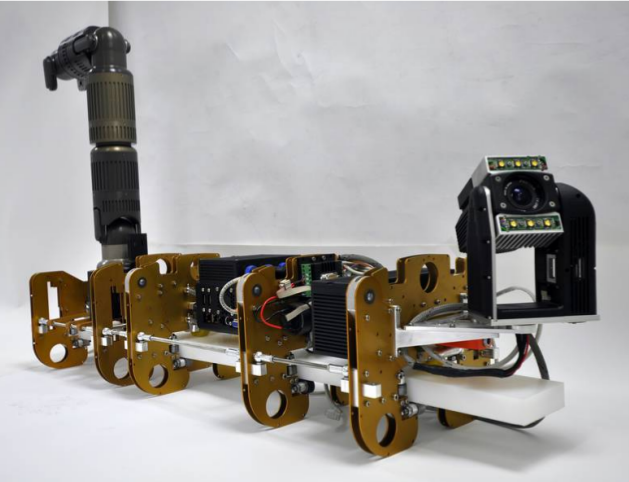
\includegraphics[height=\twosubht]{./img/artis.png}%
}
\end{figure}


\end{frame}

%------------------------------------------------

\begin{frame}
\frametitle{Motivação}
\begin{itemize}
\item DORIS:
\item Robô guiado por trilhos para monitorar e inspecionar área \textit{topside} de instalações de óleo e gás.
\end{itemize}
\begin{figure}
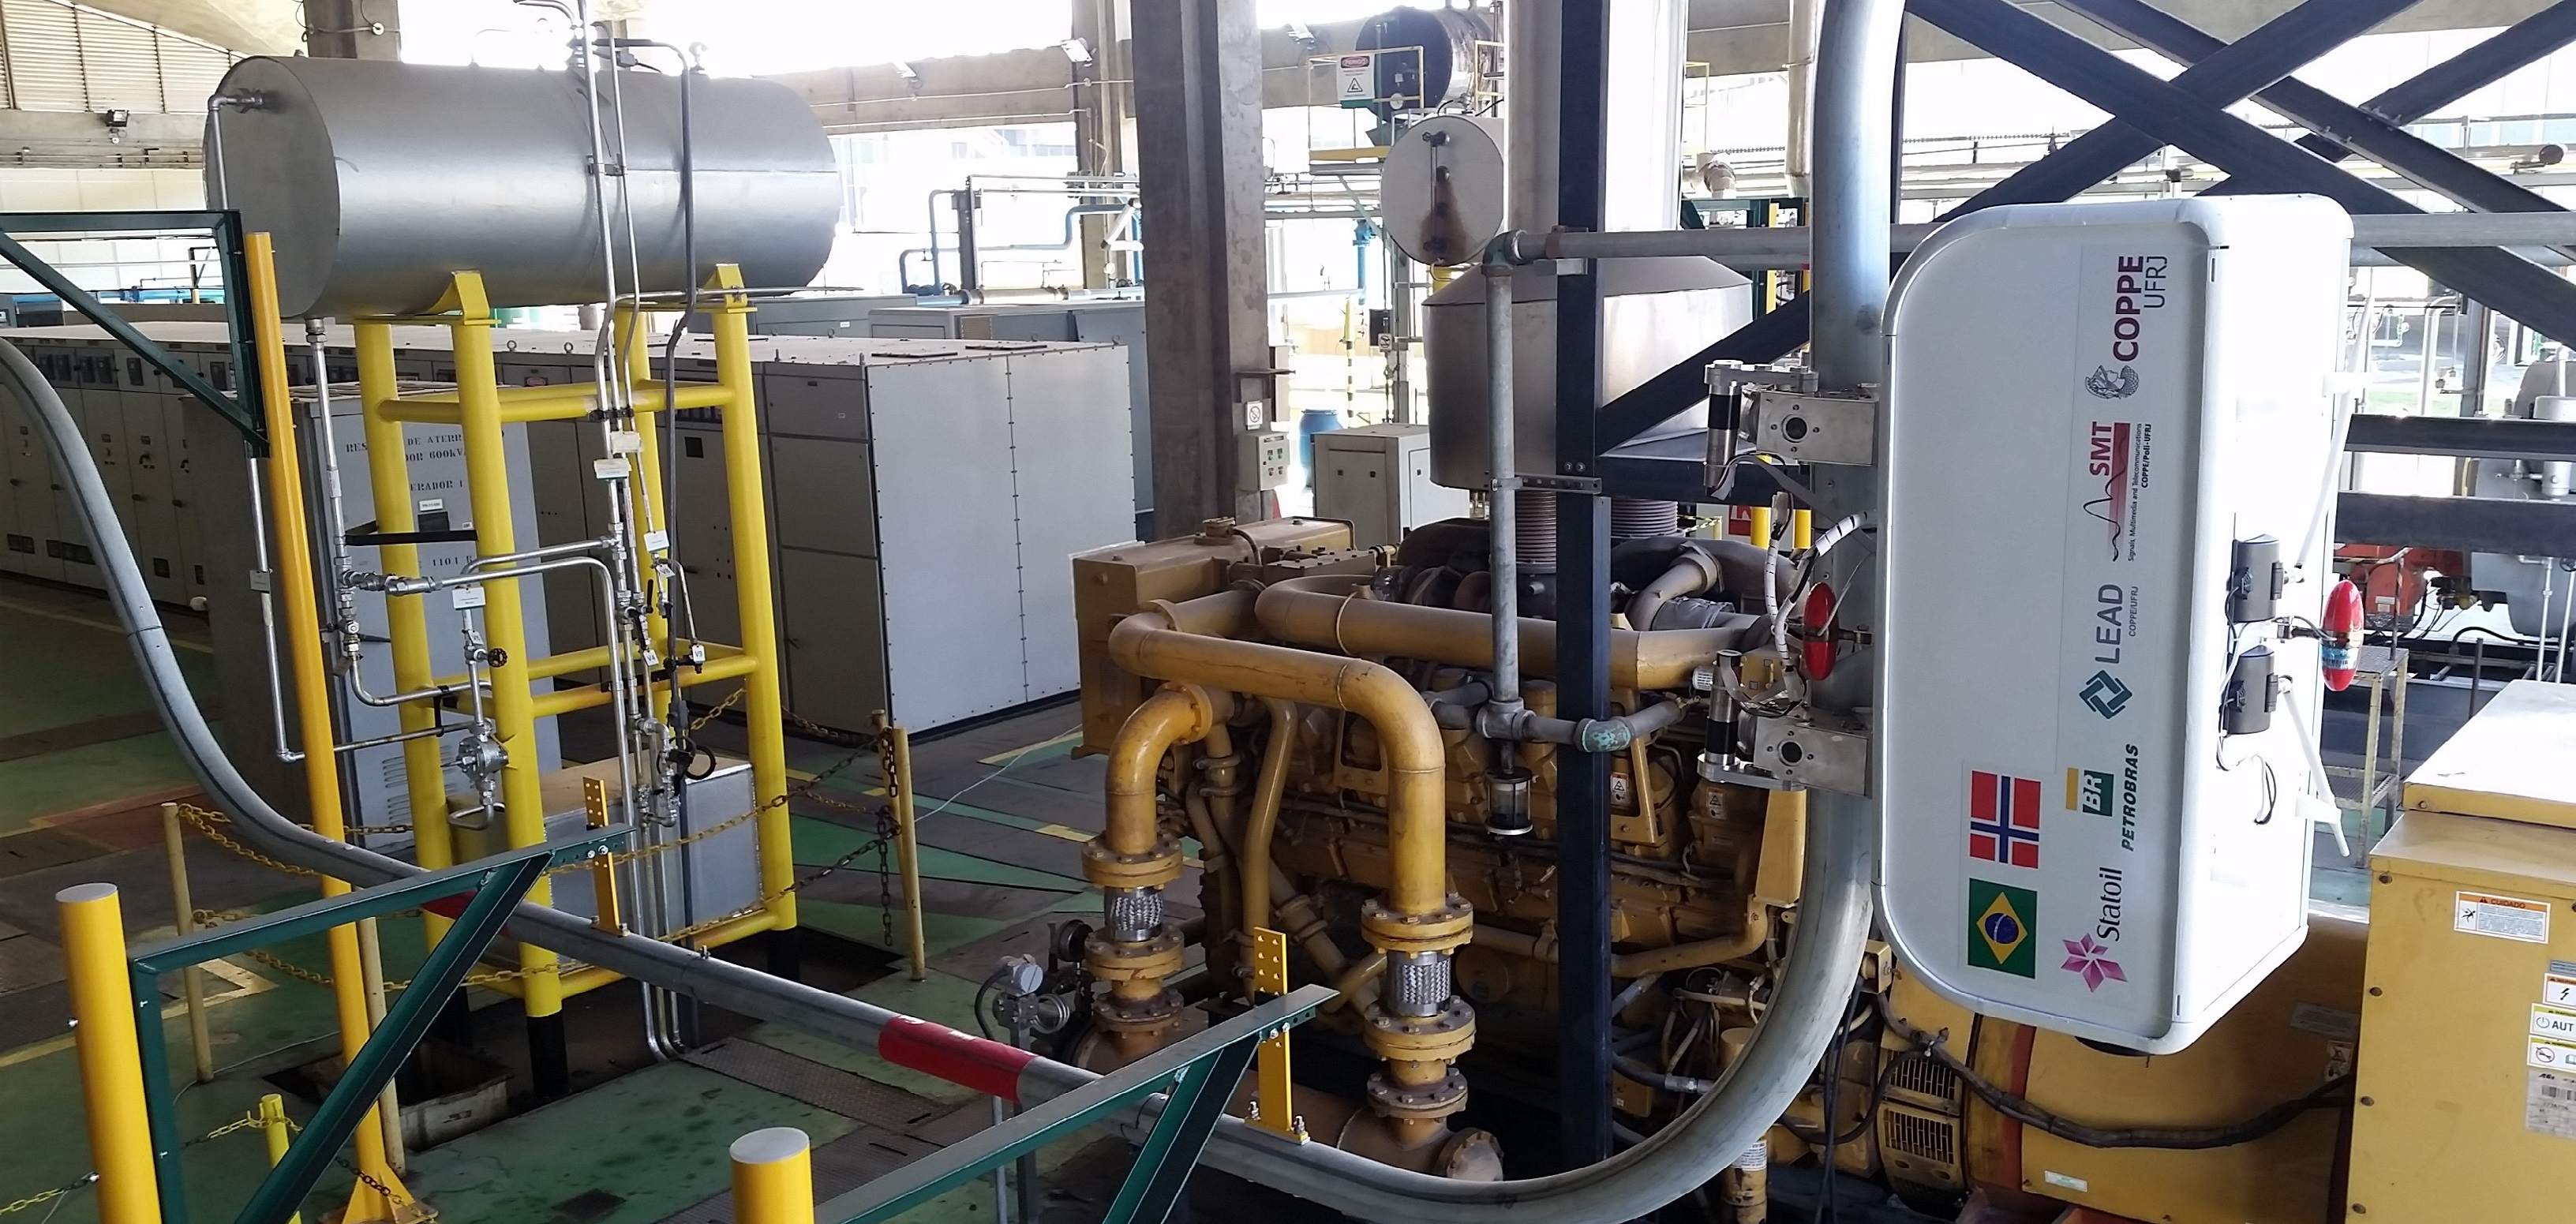
\includegraphics[width=0.8\linewidth]{./img/cenpes_field.jpg}
\caption{DORIS em operação no CENPES}
\end{figure}
\end{frame}

%------------------------------------------------


\begin{frame}
\frametitle{DORIS}
\begin{figure}
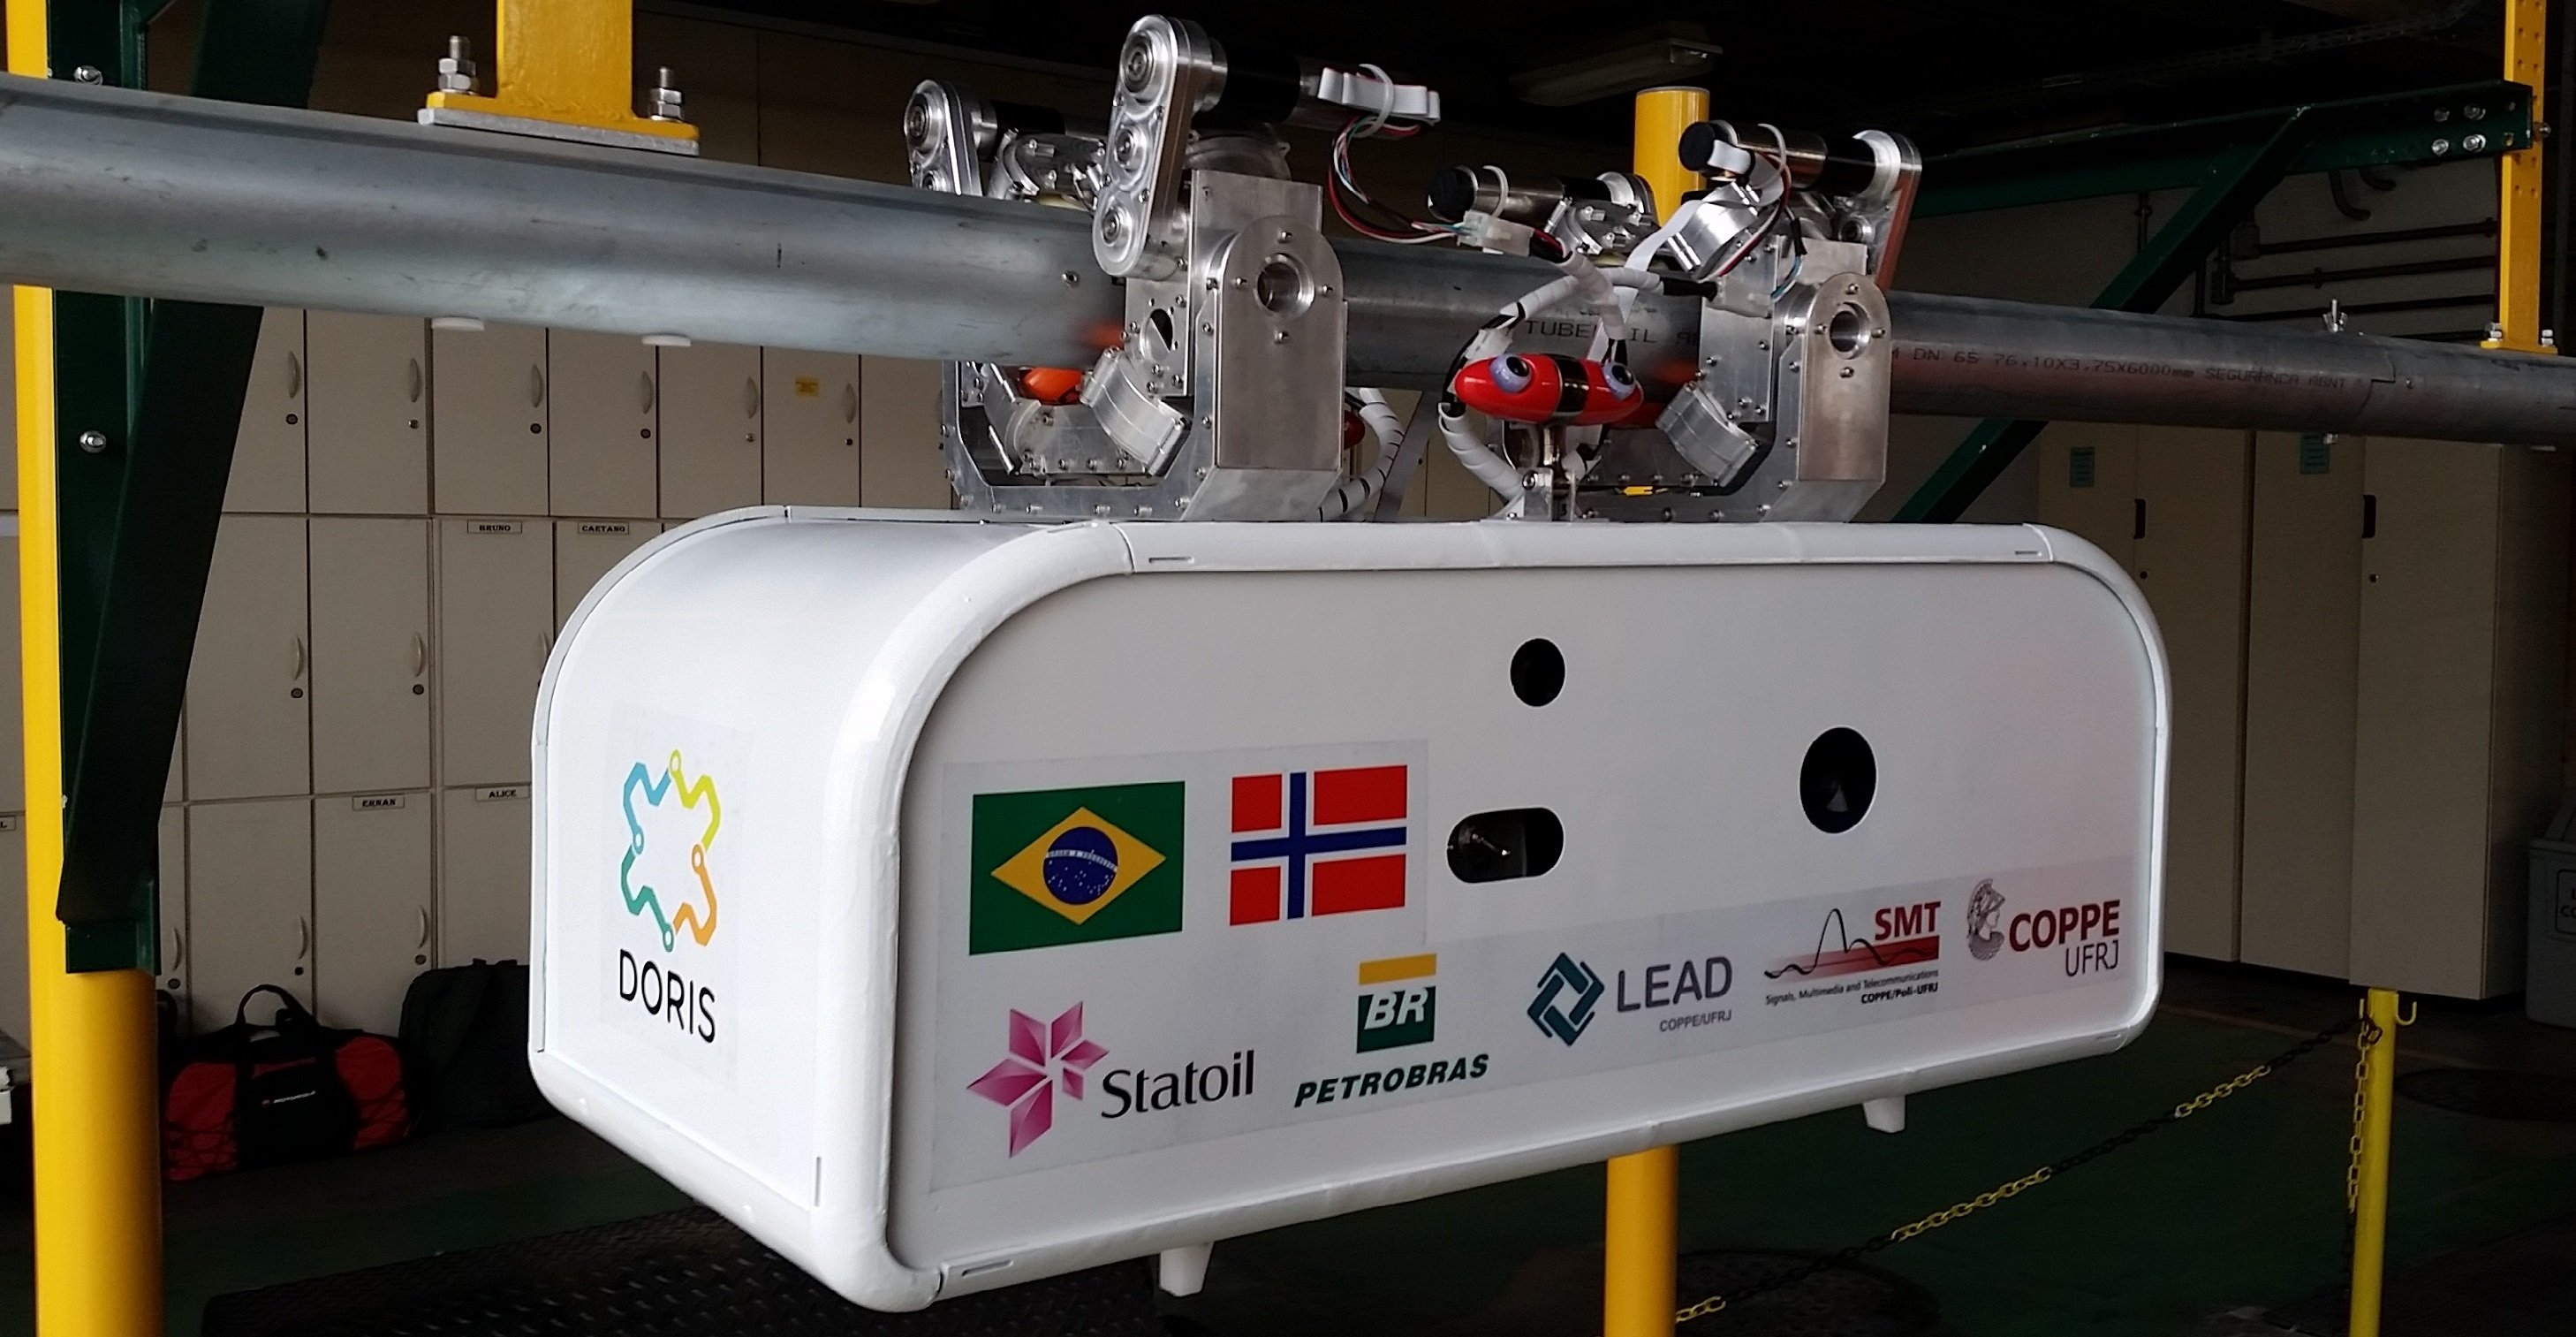
\includegraphics[width=0.65\linewidth]{./img/doris_robot.jpg}
\caption{DORIS em operação no CENPES}
\end{figure}
\begin{itemize}
\item Monitorar perfis de temperatura.
\item Supervisão de pessoal não autorizado.
\item Inspeção de padrões de vibração.
\item Interação com interfaces touchscreen na plataforma.
\end{itemize}
\end{frame}

%------------------------------------------------

\begin{frame}
\frametitle{Manipulador TETIS}
\begin{itemize}
\item Mover a câmera acoplada ao efetuador.
\item Posicionar o sensor de vibração corretamente sobre superfície de um equipamento na plataforma.
\item Interagir com touchscreens. 
\end{itemize}
\begin{figure}
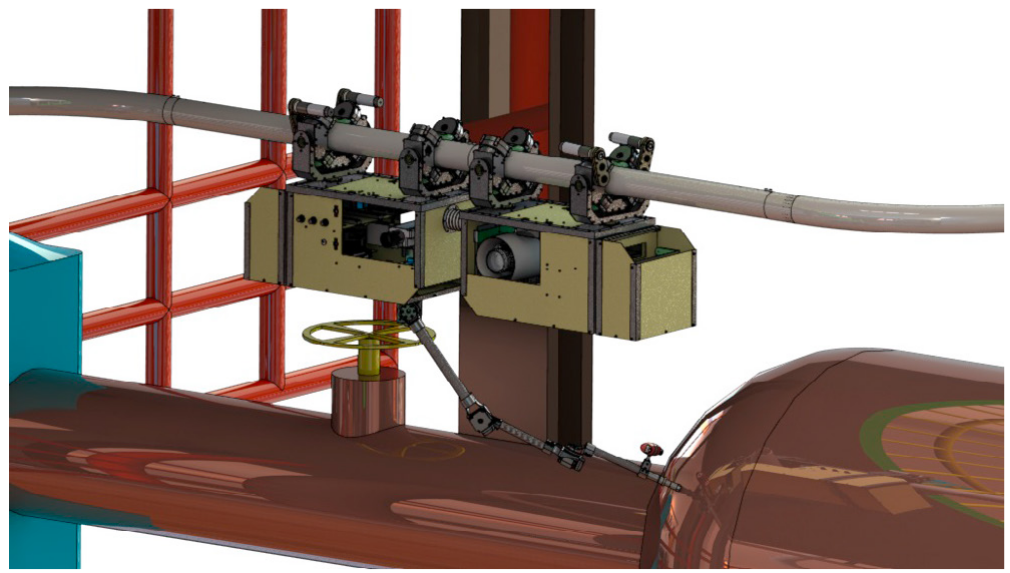
\includegraphics[width=0.7\linewidth]{./img/doris_manip.png}
\end{figure}
\end{frame}


%------------------------------------------------

\begin{frame}
\frametitle{Objetivos}
\begin{itemize}
\item Elaborar modelo cinemático e estratégias de controle. %rastreamento de trajetória
\item Controle por servo-visão na configuração \textit{eye-in-hand} onde o objetivo é rastrear um objeto de interesse: máquina a ser inspecionada.
\item Controle de força utilizando o sensor no efetuador.
\item Desenvolver a partir do RobotGUI o software que implementa o controle do TETIS. %FALAR O QUE E ROBOTGUI
\end{itemize}
\end{frame}
%------------------------------------------------


\begin{frame}

\frametitle{Cinemática Direta} % PARA MODELAR UM MANIPULADOR UTILIZASE 
\begin{itemize}
\item Manipulador: composto de Elos e Juntas 
\item Juntas podem ser prismáticas ou de revolução
\begin{figure}
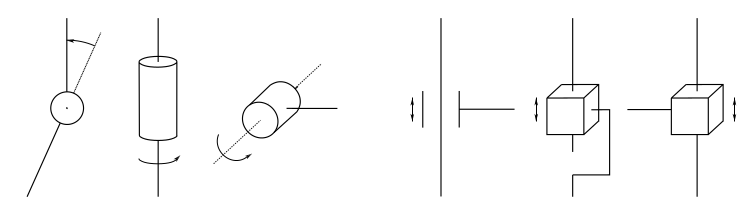
\includegraphics[width=0.8\linewidth]{./img/joints.png}
\end{figure}
\item Cadeia cinemática: Uma sequência de juntas conectadas por corpos rígidos (elos).
%FALAR SOBRE SISTEMAS DE COORDENADAS solidário EM CADA elo....
\begin{block}{Cinemática Direta}
\begin{equation} \label{eq:cinedireta}
{T}_{0n}({q}) = {T}_{01}(q_1) {T}_{12}(q_{2}) {\dots} {T}_{n-1,n}(q_n)
\end{equation}
\end{block}
\end{itemize}
\end{frame}


\begin{frame}
\frametitle{Cinemática Direta - TETIS}
Convenção Denavit-Hartenberg
\begin{figure}
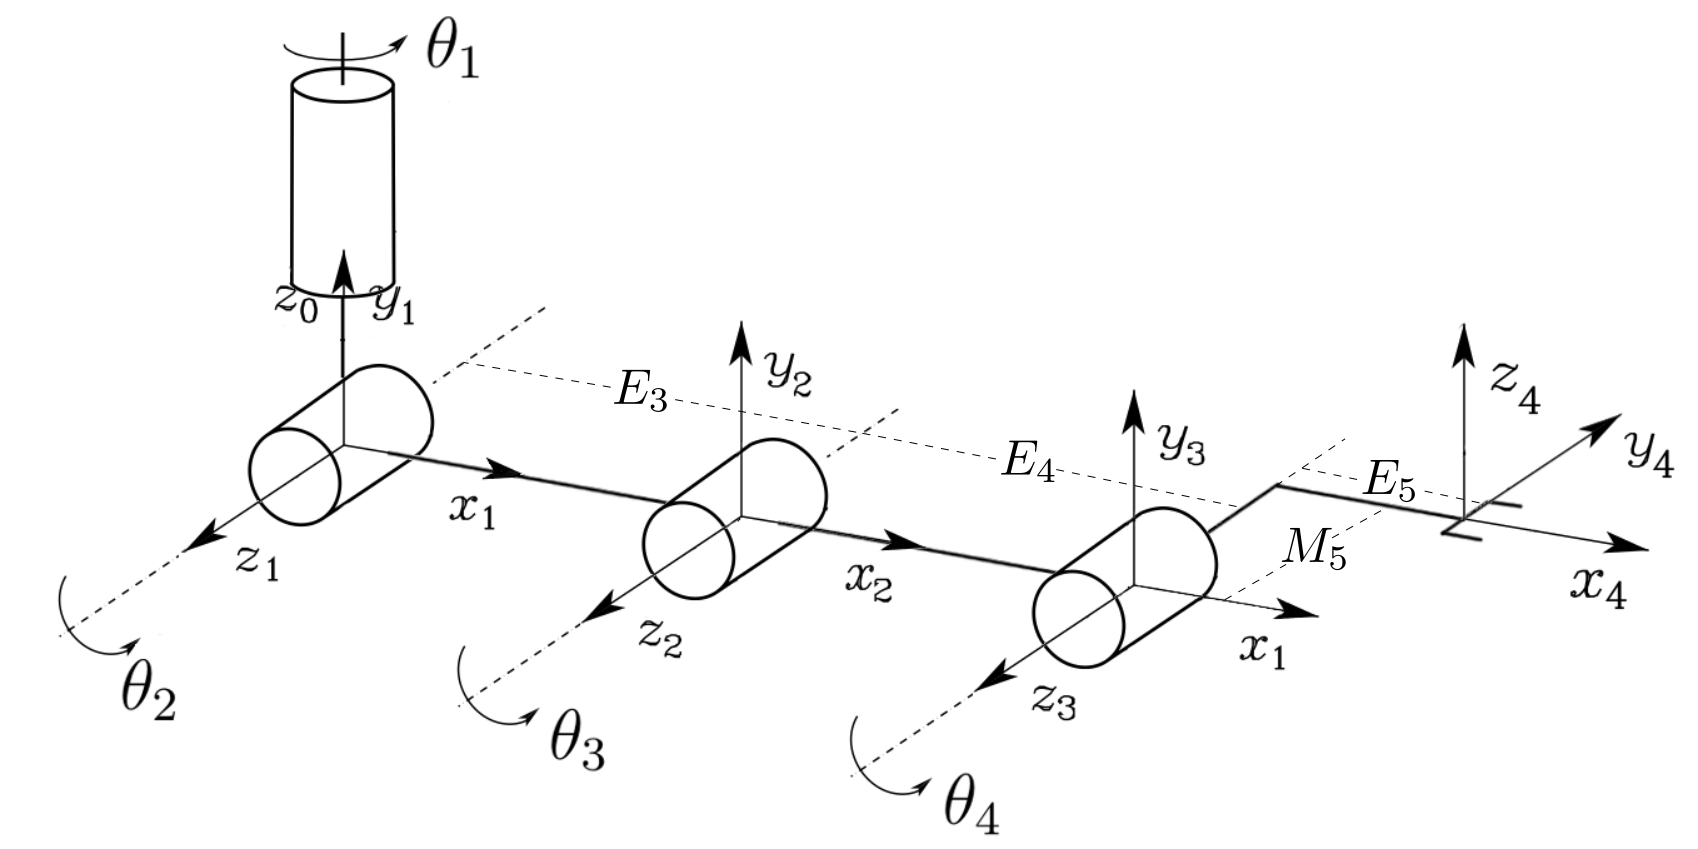
\includegraphics[width=0.8\linewidth]{./img/model2.png}
\end{figure}
\end{frame}

\begin{frame}
\frametitle{Cinemática Direta - TETIS}

\begin{figure}
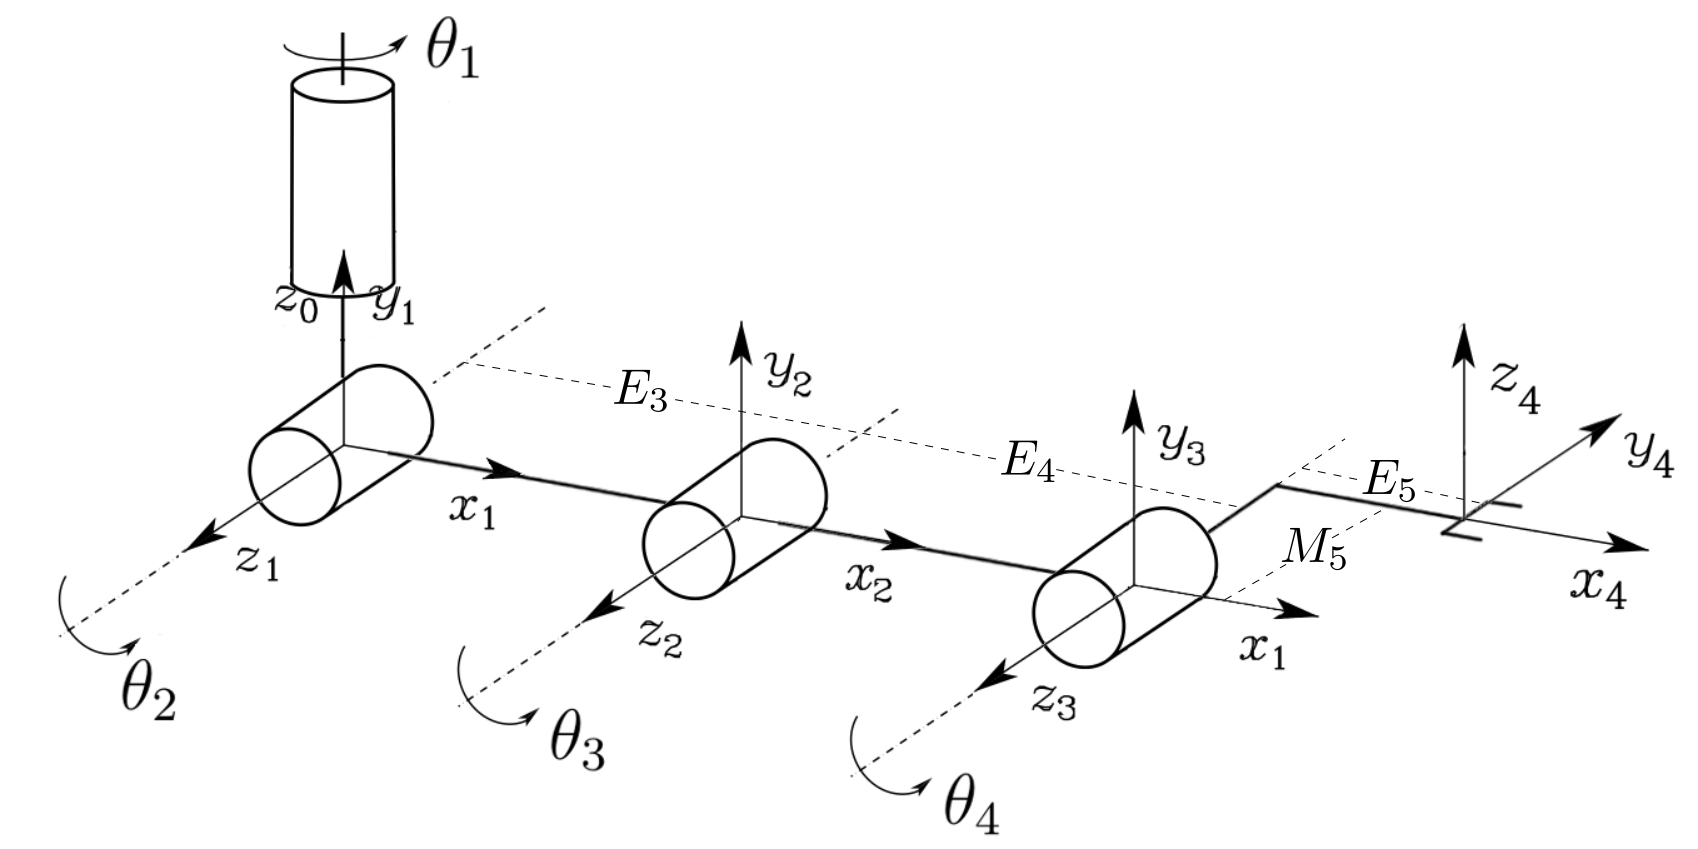
\includegraphics[width=0.5\linewidth]{./img/model2.png}
\end{figure}

\begin{table}
\begin{tabular}{rrrrr} 	
\toprule
Elo & $a_i$ & $\alpha_i$ & $d_i$  & $\theta_i$ \\ 
\midrule
1   & 0     & $\pi/2$    & 0      & $\theta_1$ \\
2   & $E_3$ & 0          & 0      & $\theta_2$ \\
3   & $E_4$ & 0          & 0      & $\theta_3$ \\
4   & $E_5$ & $-\pi/2$   & $-M_5$ & $\theta_4$ \\ 
\bottomrule
\end{tabular}
\caption{Parâmetros Denavit-Hartenberg: Manipulador TETIS}
\end{table}
\end{frame}


\begin{frame}
\frametitle{Cinemática Direta}

Para dois sistemas de coordenadas consecutivos:

\begin{equation}
{R}_{i-1,i} = {R}_z(\theta_i){R}_x(\alpha_i)
\end{equation}

\begin{gather}
{\vec{p}}_{i-1,i} = d_i {\vec{z}}_{i-1} + a_i {\vec{x}}_i \\
({\vec{p}}_{i-1,i})_{i-1} = d_i ({\vec{z}}_{i-1})_{i-1} + a_i ({\vec{x}}_i)_{i-1} \\
({\vec{p}}_{i-1,i})_{i-1} = d_i ({\vec{z}}_{i-1})_{i-1} + a_i {R}_{i-1,i}({\vec{x}}_i)_{i} 
\end{gather}

\begin{equation}
T_{i-1,i} = \m{
    R_{i-1,i}       &  ({\vec{p}}_{i-1,i})_{i-1} \\
    0_{1 \times 3}  &                             1
}
\end{equation}

\begin{equation} \label{eq:cinedireta}
{T}_{0n}({q}) = {T}_{01}(q_1) {T}_{12}(q_{2}) {\dots} {T}_{n-1,n}(q_n)
\end{equation}

\end{frame}

\begin{frame}
\frametitle{Espaços de Controle}
Definição dos espaços onde o controle será aplicado.

\begin{block}{Espaço operacional}
\begin{equation} \label{eq:op_space}
{x}_e = \m{ {p}_e \\ {\phi}_e}
\end{equation}
onde ${p}_e \in \mathbb{R}^3$ é a posição cartesiana e ${\phi}_e$ é uma representação mínima da orientação.
\end{block}

\begin{block}{Espaço das juntas}
\begin{equation} \label{eq:joint_space}
{q} = \m{q_1 \\ \vdots \\ q_n}
\end{equation} 
onde se junta é de revolução $q_i = \theta_i$, se é prismática $q_i = d_i$.
\end{block}
\end{frame}

\begin{frame}
\frametitle{Espaços de Controle - TETIS}

\begin{block}{Espaço operacional}

\begin{equation} \label{eq:operational_space}
{x_e} = \m{{p}_e \\ \phi_e}
\end{equation}
onde ${p}_e \in \mathbb{R}^3$ é a posição cartesiana e ${\phi}_e$ dado por
\begin{equation} \label{eq:orientacao} %FALAR QUE È 4DOF, orientação arbitrária
\phi_e = -(\theta_2 + \theta_3 + \theta_4)
\end{equation}
\end{block}

\begin{block}{Espaço das juntas}
\begin{equation} \label{eq:joint_space}
{q} = \m{q_1 \\ q_2 \\ q_3 \\ q_4} = \m{ \theta_1 \\ \theta_2 \\ \theta_3 \\ \theta_4}
\end{equation} 
onde todas as juntas são de revolução $q_i = \theta_i$.
\end{block}
\end{frame}

\begin{frame}
\frametitle{Cinemática Diferencial}
\begin{block}{Jacobiano analítico de posição}
\begin{equation} \label{eq:jacob_pos}
\dot{{p}}_e = \frac{\partial {p}_e }{\partial {q}} {\dot{q}} = {J}_{ap} ({q}) {\dot{q}} 
\end{equation}
\end{block}

\begin{block}{Jacobiano analítico de orientação}
\begin{equation} \label{eq:jacob_or}
\dot{{\phi}}_e = \frac{\partial {\phi}_e}{\partial {q}} {\dot{q}} = {J}_{a\phi}({q}){\dot{q}}
\end{equation}
\end{block}

\begin{block}{Jacobiano analítico}
\begin{equation} \label{eq:jacoba}
\dot{x}_e = \m{ \dot{p}_e \\ \phi_e } = \m{ J_{a_p}(q) \\ J_{a_\phi}(q)} {\dot{q}} = {J}_a ({q}) \dot{{q}}
\end{equation}
\end{block}
\end{frame}


\begin{frame}
\frametitle{Controle Cinemático}
Assume-se que:
\begin{itemize}
\item Elevados fatores de redução nas juntas.
\item Baixas velocidades na realização das tarefas.
\item Existência uma malha de controle de velocidade de alto desempenho em cada junta.
\end{itemize}
As juntas devem ser capazes de reproduzir bem comandos de velocidade:
\[ {u} \approx \dot{{q}}\]
\end{frame}

\begin{frame}
\frametitle{Controle Cinemático}
O problema de controle consiste em rastrear uma trajetória ${x}_d(t)$, de modo que  ${x}_e$ atinja ${x}_d(t)$ em $t \to \infty$.
\begin{equation}
{\dot{e}} = {\dot{x}}_d - {\dot{x}_e}
\end{equation}
\begin{equation}
{\dot{e}} = {\dot{x}}_d - {J}_a({q})\dot{{q}}
\end{equation}
Assumindo que ${J}_a({q})$ é quadrada e não singular, a escolha da lei de controle
\begin{equation}
{u} = {J}_a^{-1}({q})\bar{{u}}
\end{equation}
onde
\begin{equation}
\bar{{u}} = \dot{{x}}_d + {K_t} ({x}_d - {x}_e)
\end{equation}
\end{frame}

\begin{frame}
\frametitle{Controle Cinemático}
Dinâmica do erro:
\begin{equation}
\dot{{e}} + {K_t} {e} = 0
\end{equation}
Sistema é assintoticamente estável, com $e \rightarrow 0$ quando $t \to \infty$.
\begin{figure}[h!]
\centering {\usetikzlibrary{positioning}
\usetikzlibrary{shapes,arrows}
\tikzstyle{block} = [draw, fill=blue!20, rectangle, 
    minimum height=3em, minimum width=2em]
\tikzstyle{sum} = [draw, fill=blue!20, circle, node distance=1cm]
\tikzstyle{input} = [coordinate]
\tikzstyle{output} = [coordinate]   
\tikzstyle{pinstyle} = [pin edge={to-,thin,black}]

\tikzstyle{blockbig} = [draw, fill=white, rectangle, 
    minimum height=6em, minimum width=3em]
\tikzset{
block/.style = {draw, fill=white, rectangle, minimum height=3em, minimum width=3em},
tmp/.style  = {coordinate}, 
sum/.style= {draw, fill=white, circle, node distance=1cm},
input/.style = {coordinate},
output/.style= {coordinate},
pinstyle/.style = {pin edge={to-,thin,black}}
}



\begin{tikzpicture}[auto, node distance=2cm,>=latex']
    % We start by placing the blocks
    \node  [input, name=input2] {};
    \node at (0,-1) [input, name=input] {};
    \node [sum, right of=input] (sum) {};
    \node [block, right of=sum] (K) {${K}$};
    \node [sum, right of=K, node distance=2cm] (sum2) {};
    \node [tmp, above of =sum2, node distance=1cm] (tmp1){};
    \node [block, right of=sum2] (JA) {${J}_a^{-1}$};
    \node [block, below of=JA] (k) {${k}(\cdot)$};
    \node [block, right of=JA] (Integral) {$\int$};
    \node [tmp, above of=JA, node distance=1cm] (tmp2){};
    \node [output, right of=Integral] (output) {};

    % Once the nodes are placed, connecting them is easy. 
    \draw [draw,->] (input) -- node {${x}_d$} (sum);
    %\draw [draw,->] (input2) -- node {$u$} (sum2);
    \draw [draw,->] (input2) -- node [pos=0.1] {${\dot{x}}_d$} (tmp1)-| node [pos=0.8,anchor=left,left] {$+$} (sum2);
    \draw [->] (sum) -- node {${e}$} (K);
    \draw [->] (K) -- node {}  node[pos=0.8] {$+$} (sum2);
    \draw [->] (sum2) -- node [name=tau]  {} (JA);
    \draw [->] (JA) -- node [name=dtheta] {$\dot{{q}}$} (Integral);
    \draw [->] (Integral) -- node [name=x] {${q}$}(output);
    \draw [->] (x) |- (k);
    \draw [->] (k) -| node[pos=0.99] {$-$} node [near end] {${x}_e$} (sum);
    \draw [->] (x) |- (tmp2) -| (JA);
    %\draw [->] (output) |- (tmp1)-| node[pos=0.99] {$-$} (sum);
\end{tikzpicture}
}
\caption{Controle cinemático proporcional com feedforward}
\label{fig:controlecinematico}
\end{figure}
\end{frame}

\begin{frame}
\frametitle{Servo Visão}
\begin{itemize}
\item Controlar a posição e orientação do efetuador do manipulador em relação a um alvo utilizando características extraídas de uma imagem.
\item Servo Visão Baseada em Posição: Considera-se a posição e orientação do alvo com respeito a câmera ${T}_{ct}$ é estimada através de visão computacional. 
\end{itemize}

\begin{equation}
 {T}_{ct} =  {T}_\Delta {T}_{c't}
\end{equation}

\begin{equation}
 {T}_\Delta  =   {T}_{ct} {T}_{c't}^{-1}
\end{equation}
\end{frame}


\begin{frame}
\frametitle{Servo Visão}
\textbf{Modelo da Câmera}
\begin{figure}
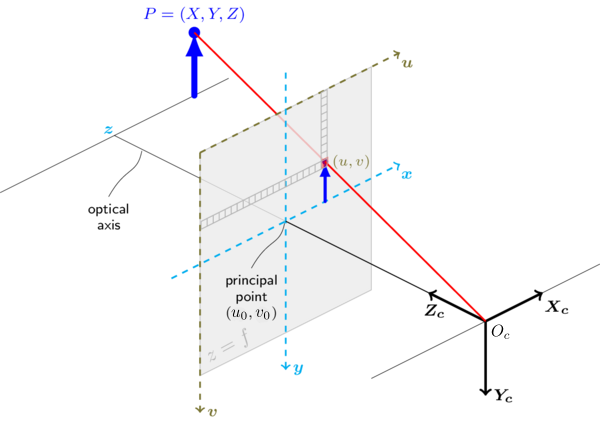
\includegraphics[height=0.75\paperheight]{./img/camera_model3.png}
\end{figure}
\end{frame}

\begin{frame}
\frametitle{Servo Visão}

\begin{block}{Projeção de perspectiva} %Colocar nome certo
% FALAR O QUE E CADA VARIAEL E SISTEMA DE COORDENADAS, parametros intrinsecos e extrinsecoss

\begin{align}\label{eq:camera_projection}
{\tilde{p}} =& 
\m {
	f/\rho_w & 0 & u_0 \\
	0        & f/\rho_h &v_0 \\
	0 & 0 & 1 \\
}
\m{  1 & 0 & 0 & 0\\
	 0 & 1 & 0 & 0\\
	 0 & 0 & 1 & 0	
}
{T}_{0c}^{-1} (\tilde{{P}})_0\\
=& {K} {P}_0 {T}_{0c}^{-1} (\tilde{{P}})_0 \\ 
=& {C} ({\tilde{P})_0}
\end{align}
onde $K$ é chamada matriz de calibração da câmera.
\end{block}
\end{frame}


\begin{frame}
\frametitle{Estimação da Pose}
\begin{itemize}
\item Determinar a posição e orientação ${T}_{ct}$ a partir de um conjunto de pontos característicos
\item \textit{Perspective-n-Point}
\item ViSP - Visual Servoing Platform
\begin{figure}
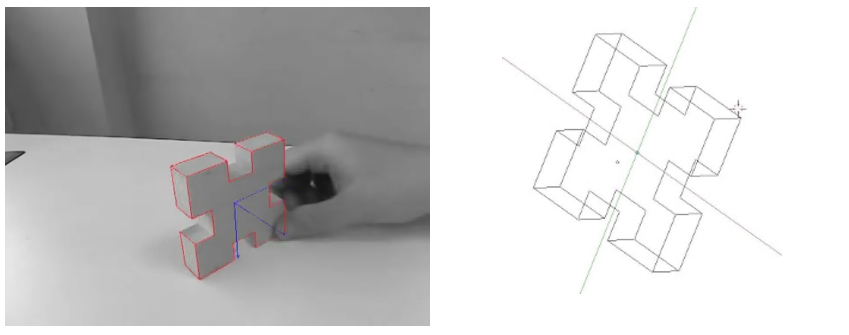
\includegraphics[width=0.75\linewidth]{./img/visp.png}
\end{figure}
\end{itemize}
\end{frame}

\begin{frame}
\frametitle{Servo Visão Baseada em Posição}
\begin{columns}[c] % The "c" option specifies centered vertical alignment while the "t" option is used for top vertical alignment

\column{.45\textwidth} % Left column and width
%\textbf{Heading}
\begin{itemize}
\item Configuração \textit{eye-in-hand}.
\item Servo Visão baseada em Posição.
\item Rastrear um QR Code
\end{itemize}

\column{.5\textwidth} % Right column and width
\begin{figure}
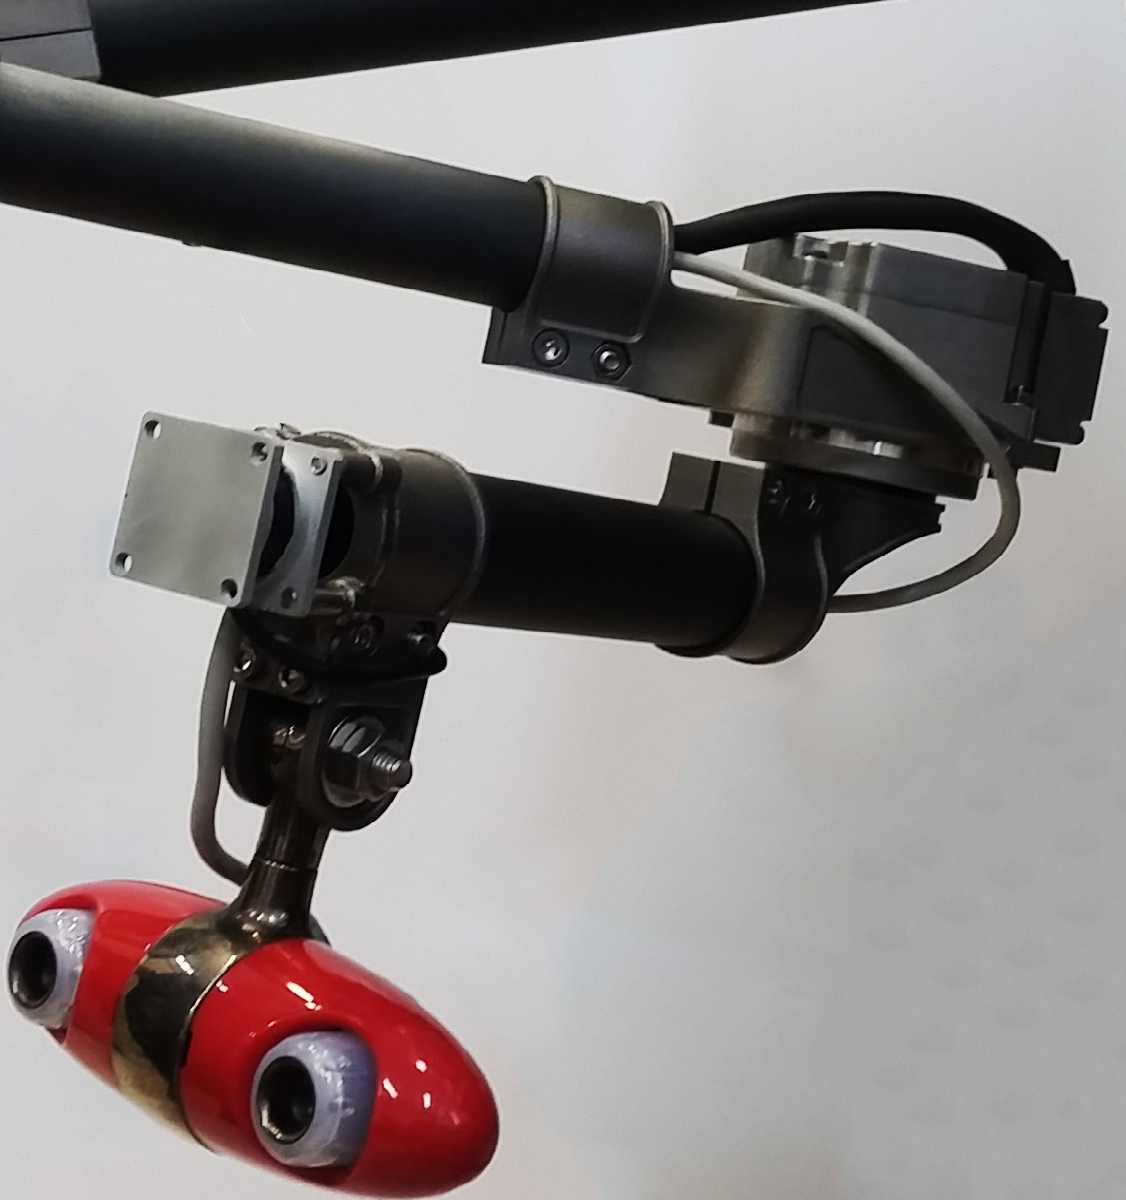
\includegraphics[width=0.5\linewidth]{./img/manip_zoom.png}
\end{figure}
\begin{figure}

\includegraphics[width=0.5\linewidth]{./img/template-qr-code-small.png}
\end{figure}
\end{columns}
\end{frame}

\begin{frame}
\frametitle{Servo Visão - Câmera Minoru}
\textbf{Matriz de calibração da câmera:  parâmetros instrínsecos.}
\begin{columns}[c] % The "c" option specifies centered vertical alignment while the "t" option is used for top vertical alignment
\column{.45\textwidth}
\begin{figure}
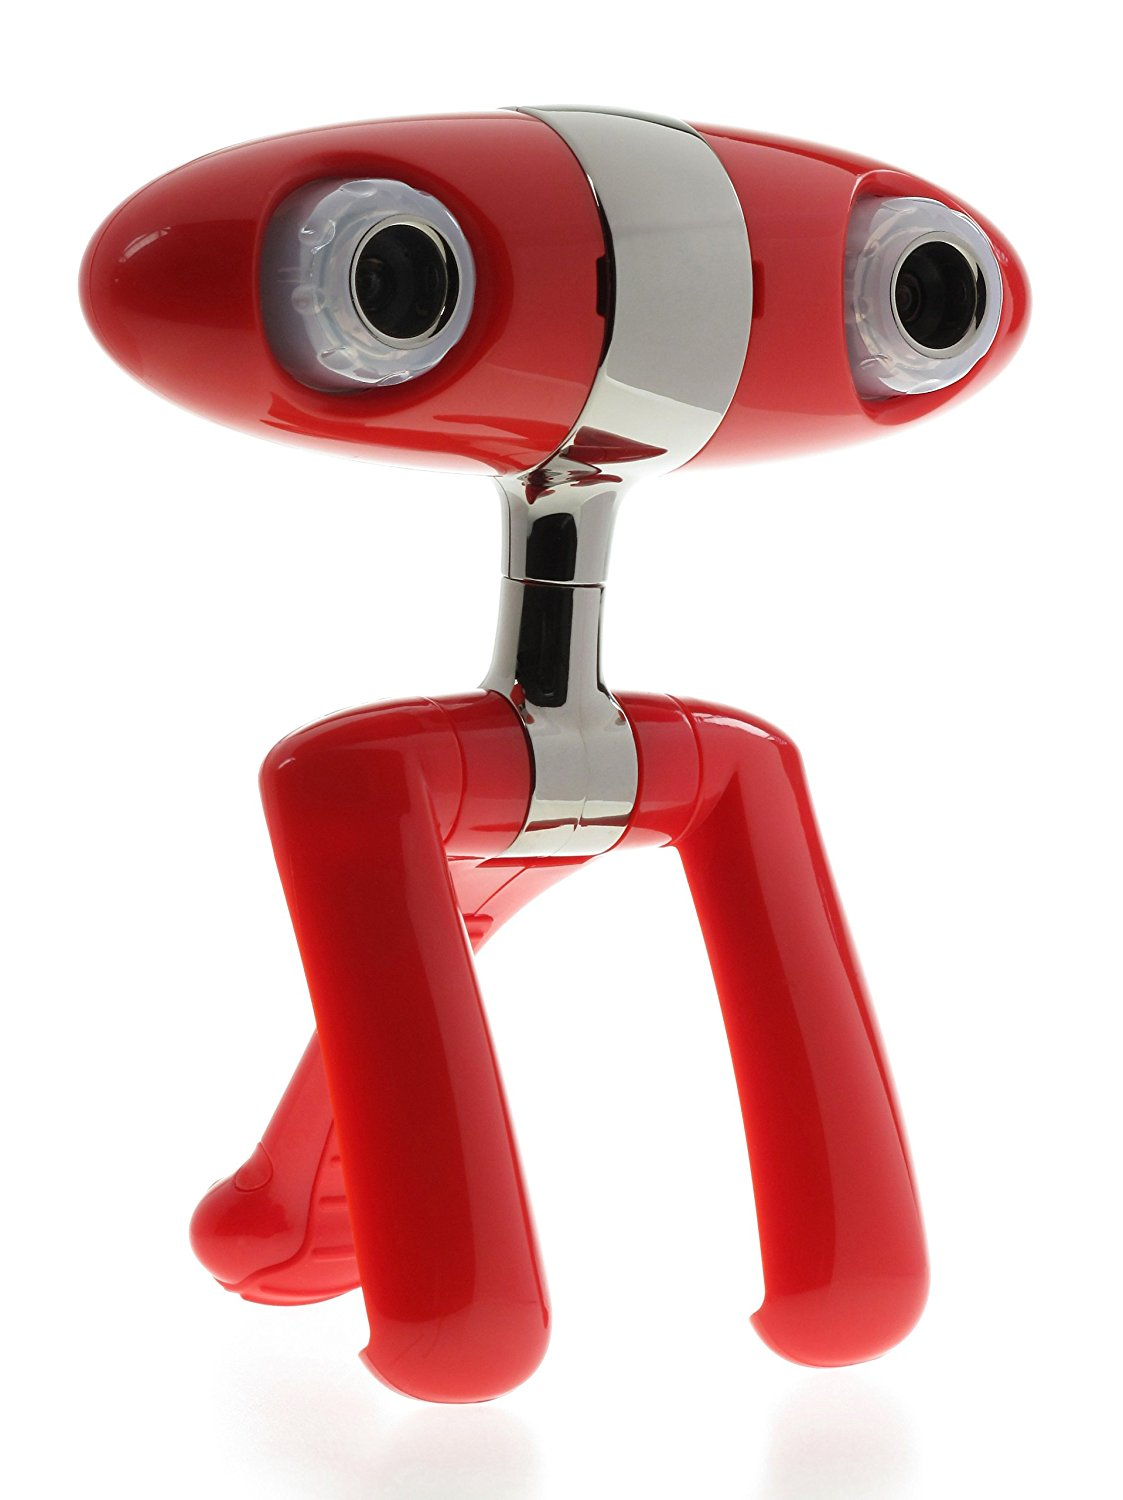
\includegraphics[width=0.5\linewidth]{./img/minoru.jpg}
\end{figure}
\column{.45\textwidth}
\begin{align*}
{K} =& \m {
	f/\rho_w & 0 & u_0 \\
	0        & f/\rho_h &v_0 \\
	0 & 0 & 1 \\
}
\\
{K} =& 
\m{
	877.62 	& 0 		& 306.53 \\
	0  		& 880.32 	& 210.12 \\
	0   	& 0 		& 1 \\	
}	
\end{align*}

%% COMO FUNCIONA A CALIBRAÇÂO?????????????????????????????????????????????
\end{columns}
\end{frame}

\begin{frame}
\frametitle{Servo Visão - TETIS}
\textbf{$T_{ct}$: Posição e orientação do alvo em relação ao sistema de coordenadas da câmera.}
\begin{columns}[c]
\column{.45\textwidth}
\begin{figure}
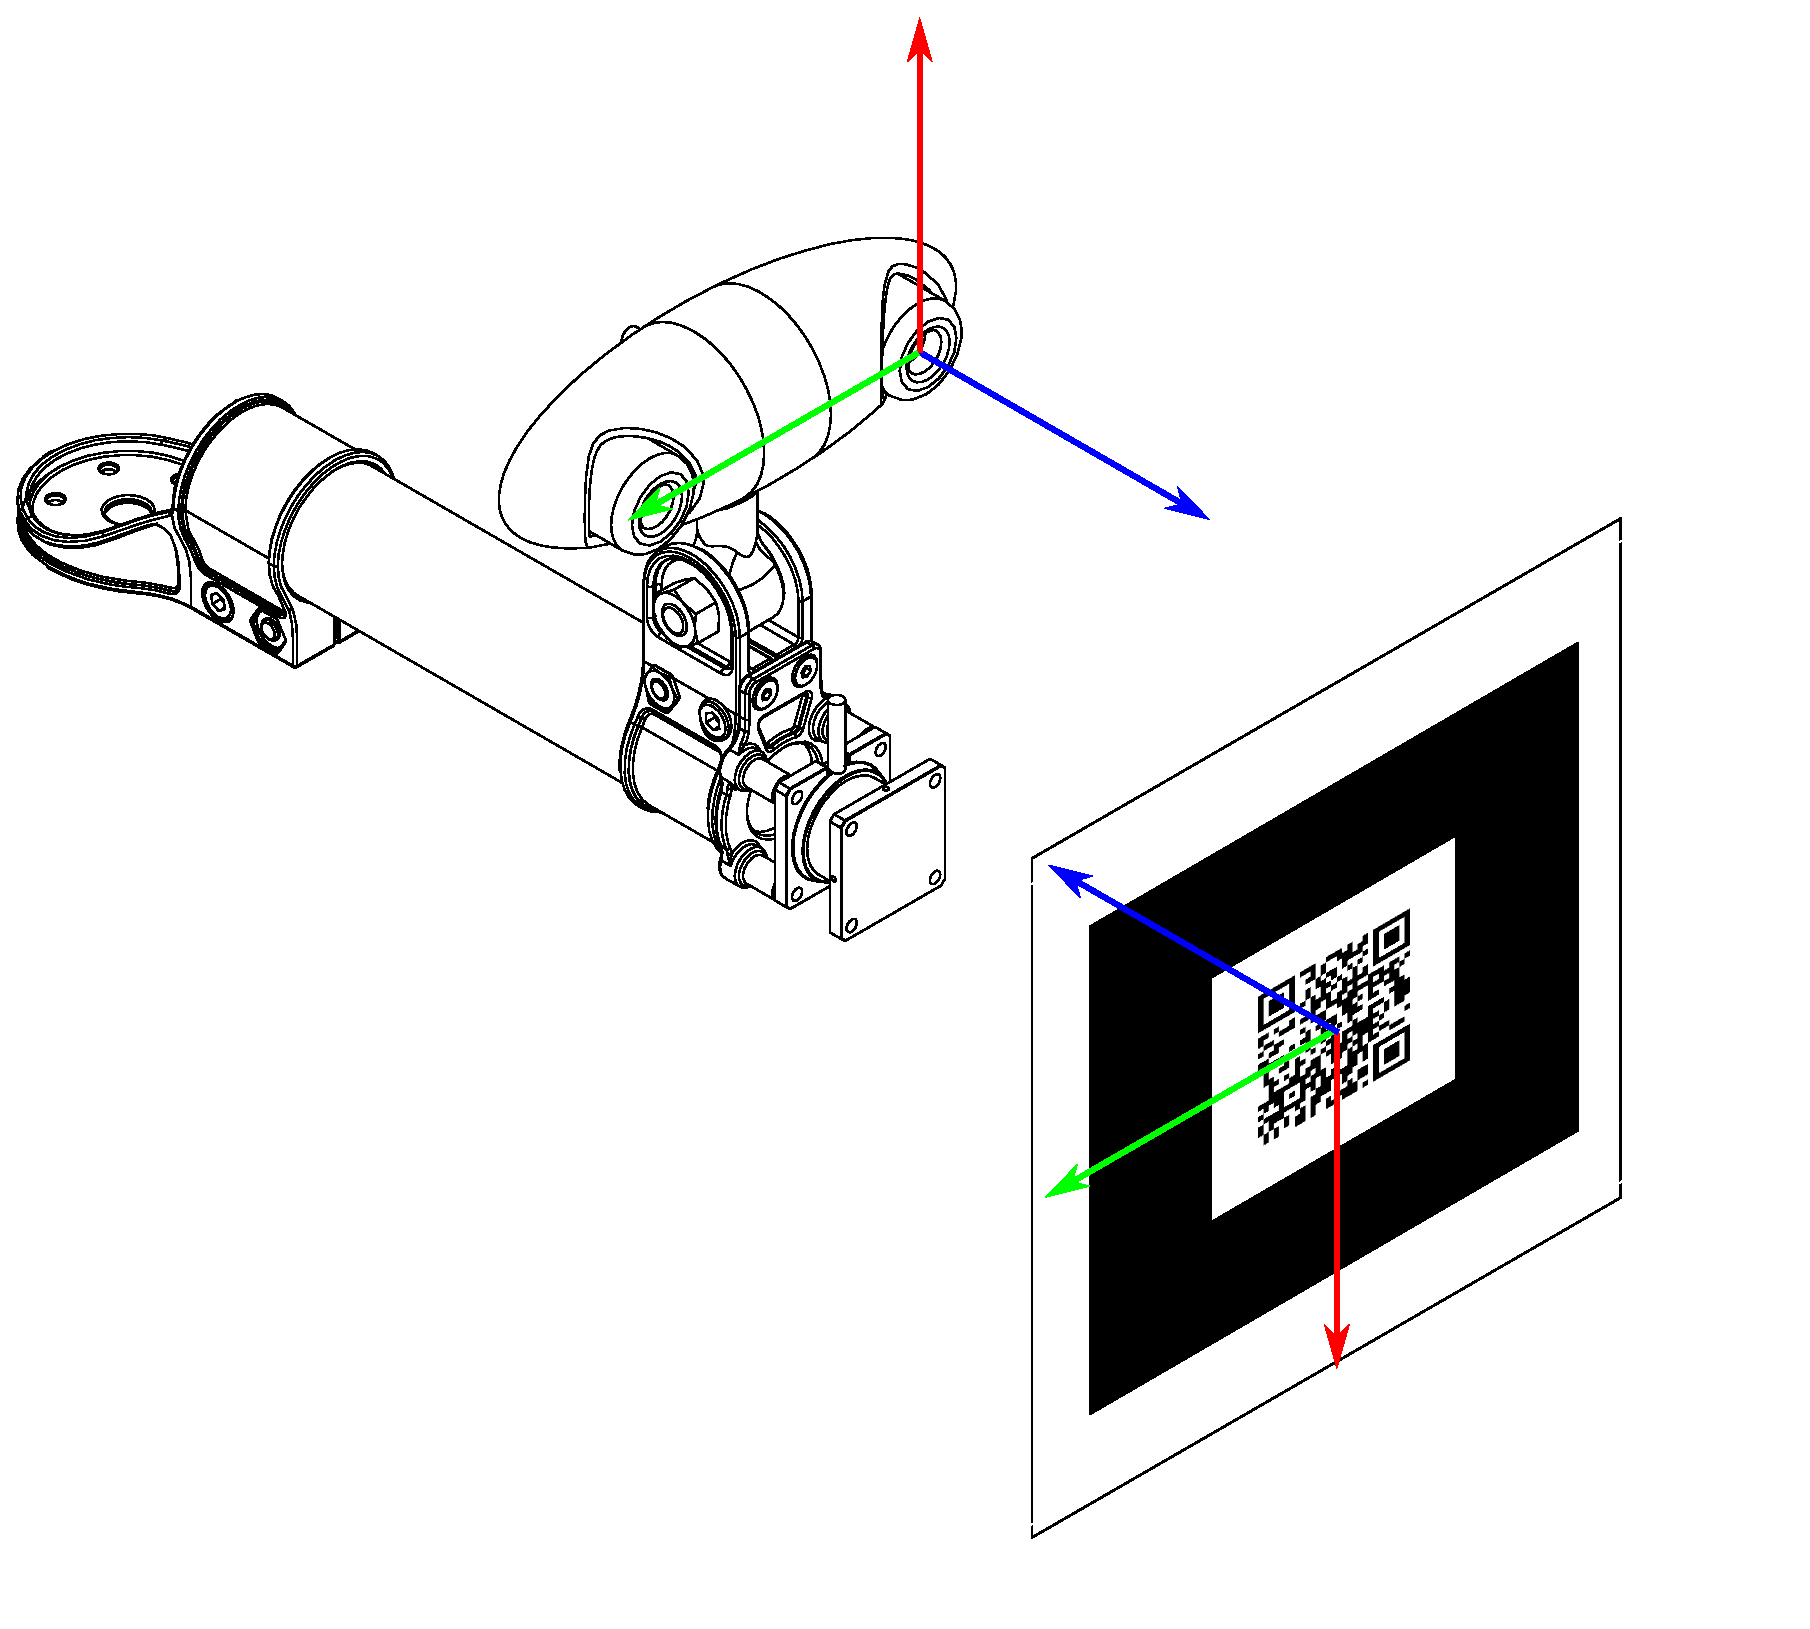
\includegraphics[width=\linewidth]{./img/camera_target.eps}
\end{figure}
\column{.45\textwidth}
\begin{equation}
T_{ct_0} = \m{
	-1 & 0 & 0  &\vdots \\
	0 & 1 & 0  & (p_{t_0})_c    \\
	0 & 0 & -1 &\vdots \\
	0 & 0 & 0 & 1
}
\end{equation}
\end{columns}
\end{frame}

\begin{frame}
\frametitle{Servo Visão - TETIS}
\textbf{$T_{ec}$: Posição e orientação da câmera em relção ao efetuador.}
\begin{columns}[c]
\column{.45\textwidth}
\begin{figure}
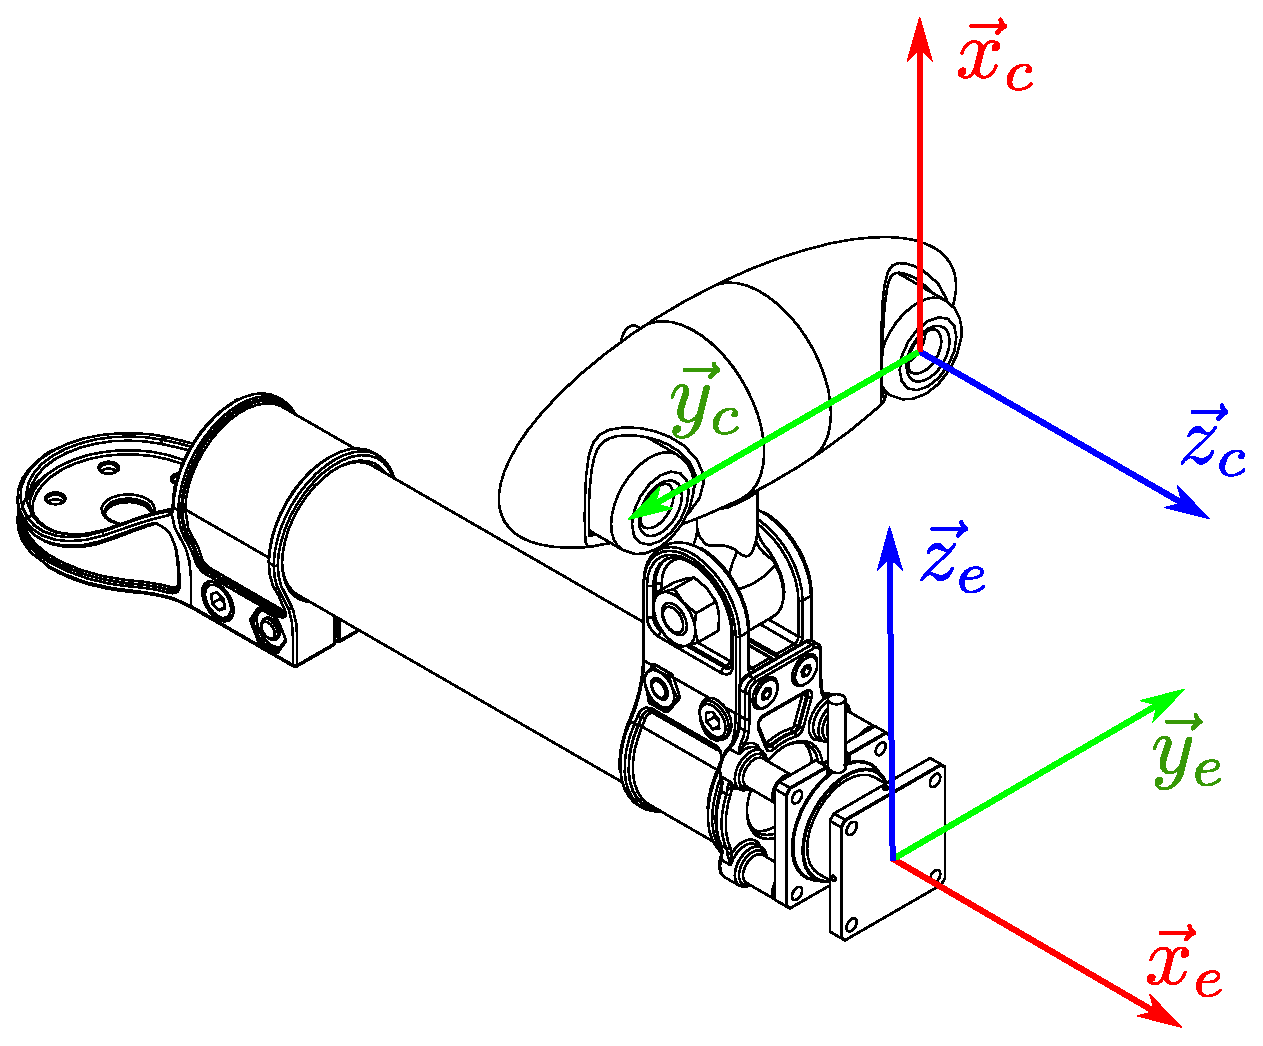
\includegraphics[width=\linewidth]{./img/effector_camera.eps}
\end{figure}

\column{.45\textwidth}
\begin{equation} \label{eq:tec}
{T}_{ec} = \m{
	0 & 0 & 1 & -30 \\
	0 & -1 & 0 & 101 \\
	1 &  0 & 0 & -43 \\
	0 &  0 & 0 &  1
}
\end{equation}
\end{columns}
\end{frame}

\begin{frame}
\frametitle{Servo Visão - TETIS}
\textbf{Orientação $\phi_t$}
\begin{figure}[!ht]
\centering
  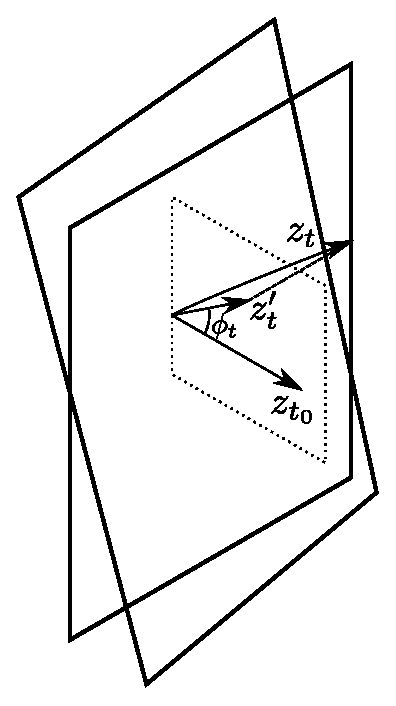
\includegraphics[width=0.3\linewidth]{./img/projection2.eps}
  \label{fig:projection}
\end{figure}%
\end{frame}

\begin{frame}
\frametitle{Servo Visão}

Após obter os valores de $(p_t)_e$ e $\phi_t$:
\begin{equation}
(x_t)_e = \m{(p_t)_e \\ \phi_t }
\end{equation} e controle fica:
\begin{align}
{e_v} &= ({x}_t)_e - ({x})_e \\
{\bar{u}_v} &= {K}_v {e}  \\
{u_v} &= ({J}_{a})_e^{-1} {e_v}
\end{align}
\end{frame}



\begin{frame}
\frametitle{Hardware - Descrição}
\begin{figure}
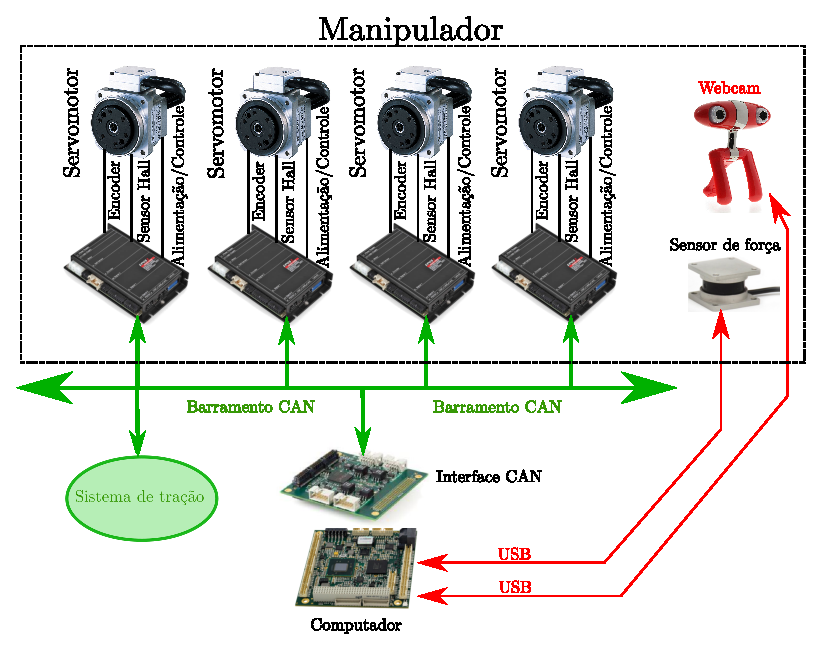
\includegraphics[width=0.8\linewidth]{./img/integration_diagram.eps}
\end{figure}
\end{frame}


\begin{frame}
\frametitle{Software - ROS}
\textbf{Robot Operating System (ROS)}
\begin{columns}[c] % The "c" option specifies centered vertical alignment while the "t" option is used for top vertical alignment

\column{.3\textwidth} % Left column and width
\begin{itemize}
\item Nodes
\item Master
\item Messages
\item Topics
\item Services
\item Nodelet
\end{itemize}

\column{.7\textwidth} % Right column and width
\begin{figure}
  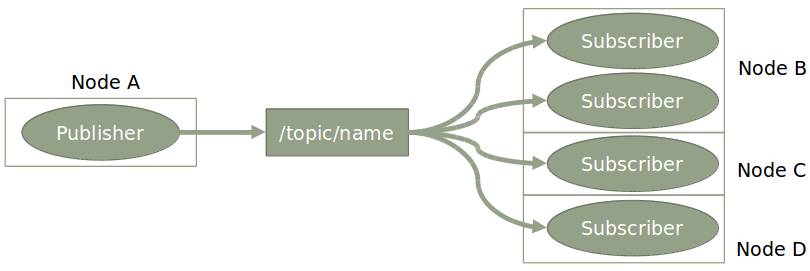
\includegraphics[width=\linewidth]{./img/topics.png}
\end{figure}
\begin{figure}
  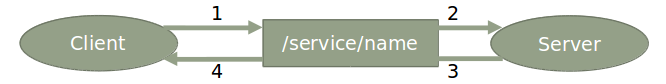
\includegraphics[width=\linewidth]{./img/services.png}
\end{figure}
\end{columns}
\end{frame}


\begin{frame}
\frametitle{Software - Topologia}
\begin{figure}
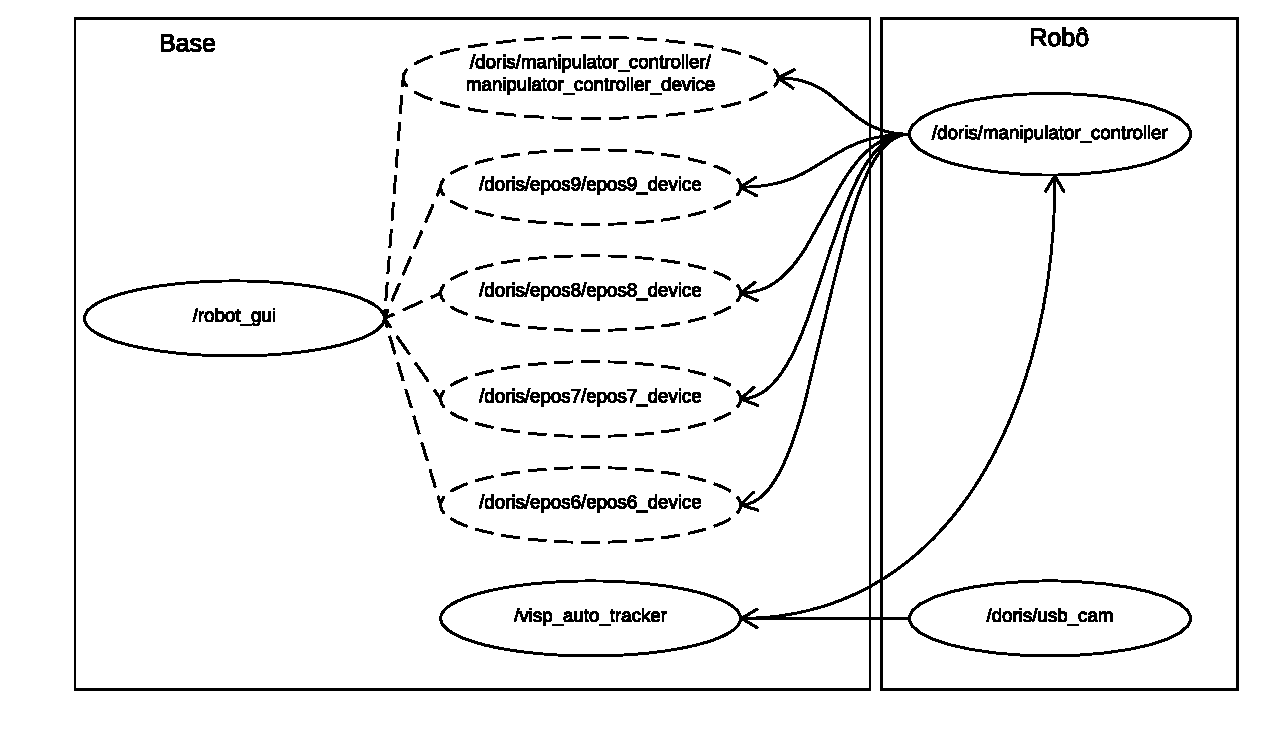
\includegraphics[width=\linewidth]{./img/nodes_simple.pdf}
\end{figure}
\end{frame}

\begin{frame}
\frametitle{Software - Interface gráfica}
\begin{figure}
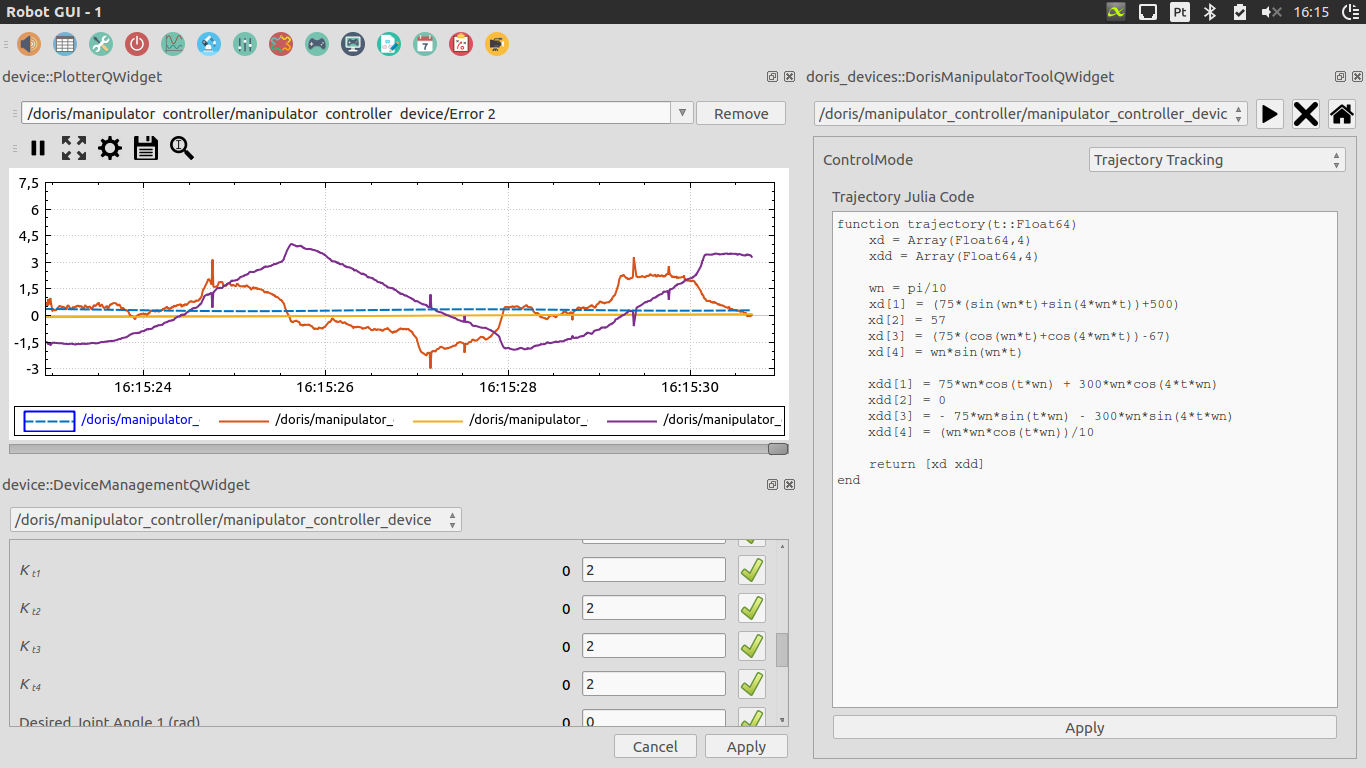
\includegraphics[width=\linewidth]{./img/screenshot/sc1.png}
\end{figure}
\end{frame}


%------------------------------------------------


\begin{frame}
\frametitle{Resultados de Simulação}
%Resultados esperados
\textbf{Resultados de simulação com ZOH de $10ms$ e ganho $K_t = 5 I$}
\begin{figure}[H]
\centering
\begin{subfigure}{.5\textwidth}
  \centering
  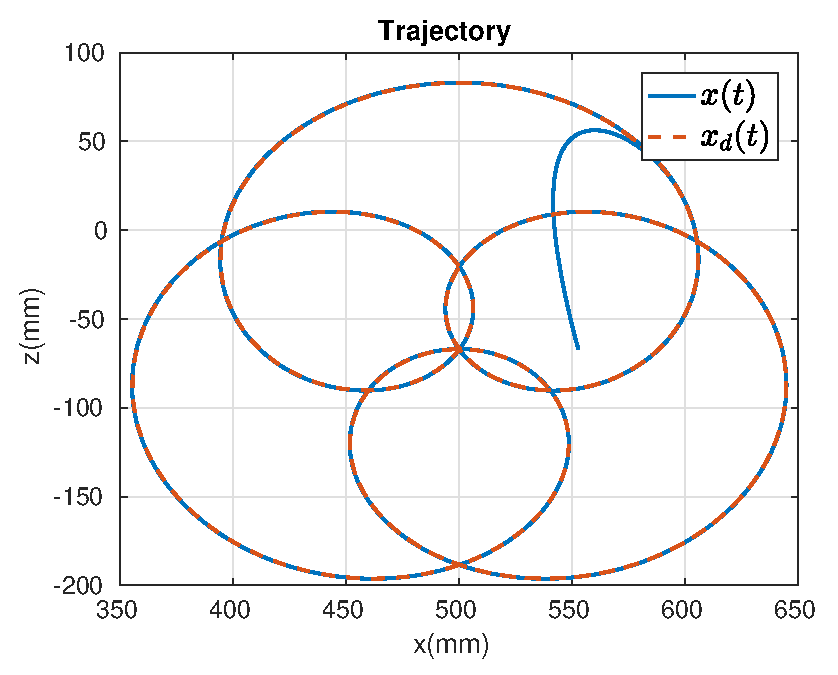
\includegraphics[width=\linewidth]{./img/simul_delay_zoh5/traj.eps}
  \caption{Plano x-z}
\end{subfigure}%
\begin{subfigure}{.5\textwidth}
  \centering
  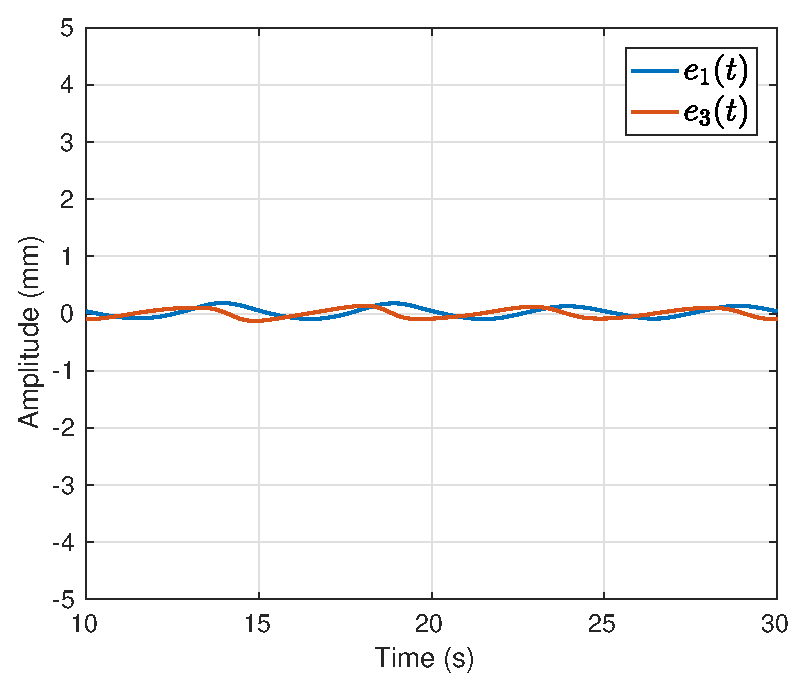
\includegraphics[width=\linewidth]{./img/simul_delay_zoh5/error.eps}
\end{subfigure}
\end{figure}%
\end{frame}


\begin{frame}
\frametitle{Resultados Experimentais - Rastreamento de Trajetória}
\textbf{Resultados experimentais com ganho $K_t = 5 I$ para trajetória 1.}
\begin{figure}[H]
\centering
\begin{subfigure}{.5\textwidth}
  \centering
  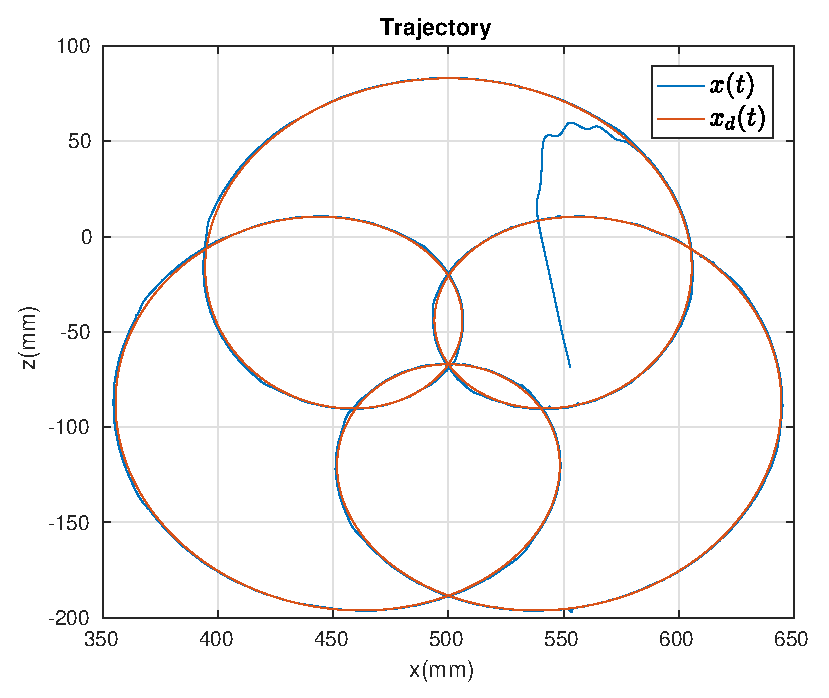
\includegraphics[width=\linewidth]{./img/traj_1_k5/traj.eps}
  \caption{Plano x-z}
\end{subfigure}%
\begin{subfigure}{.5\textwidth}
  \centering
  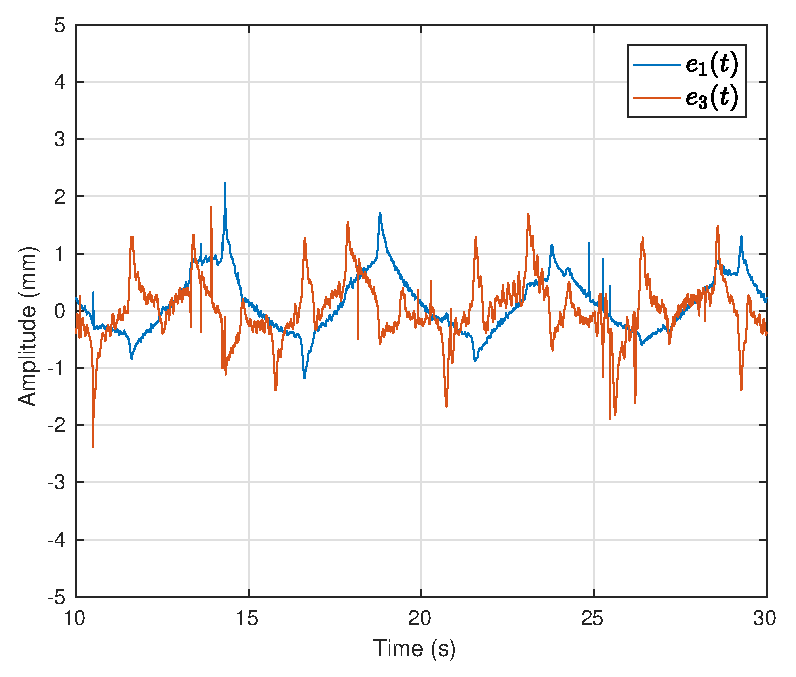
\includegraphics[width=\linewidth]{./img/traj_1_k5/error.eps}
\end{subfigure}
\end{figure}%
\begin{center}
\href{run:traject1.mp4}{\textbf{Video}}% 
\end{center}
\end{frame}


\begin{frame}
\frametitle{Resultados experimentais - Rastreamento de Trajetória}
\textbf{Resultados experimentais com ganho $K_t = 5 I$ para trajetória 2.}
\begin{figure}[H]
\centering
\begin{subfigure}{.5\textwidth}
  \centering
  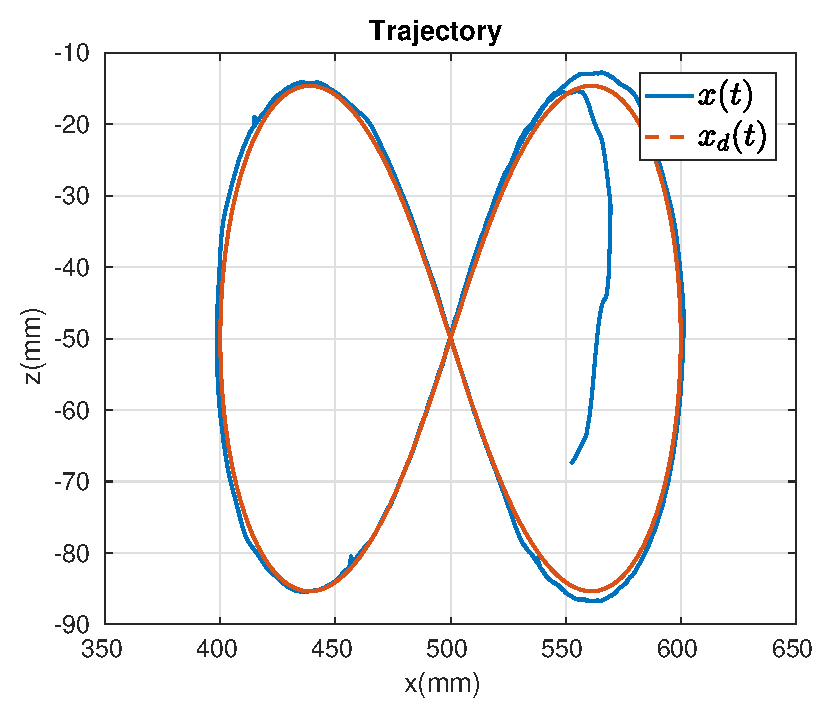
\includegraphics[width=\linewidth]{./img/traj_2_k5/traj.eps}
  \caption{Plano x-z}
\end{subfigure}%
\begin{subfigure}{.5\textwidth}
  \centering
  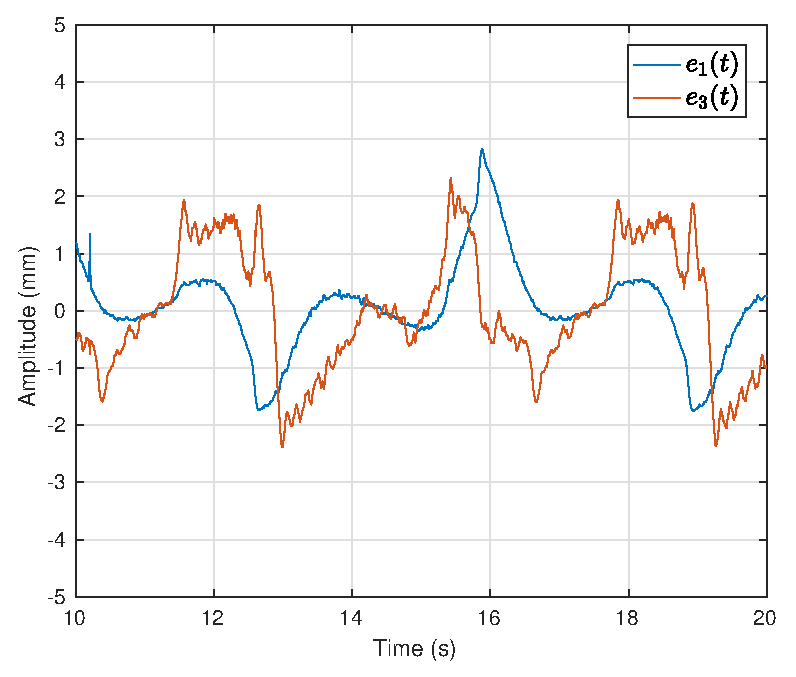
\includegraphics[width=\linewidth]{./img/traj_2_k5/error.eps}
  \caption{Erro $e_1$ e $e_2$}
\end{subfigure}
\end{figure}%\href{run:traject1.mp4}{
\begin{center}
\href{run:traject2.mp4}{\textbf{Video}}% 
\end{center}
\end{frame}

\begin{frame}
\frametitle{Resultados experimentais - Controle de Força}
\textbf{Resultados experimentais do controle de força com $k_f = 100$.}
\begin{figure}[H]
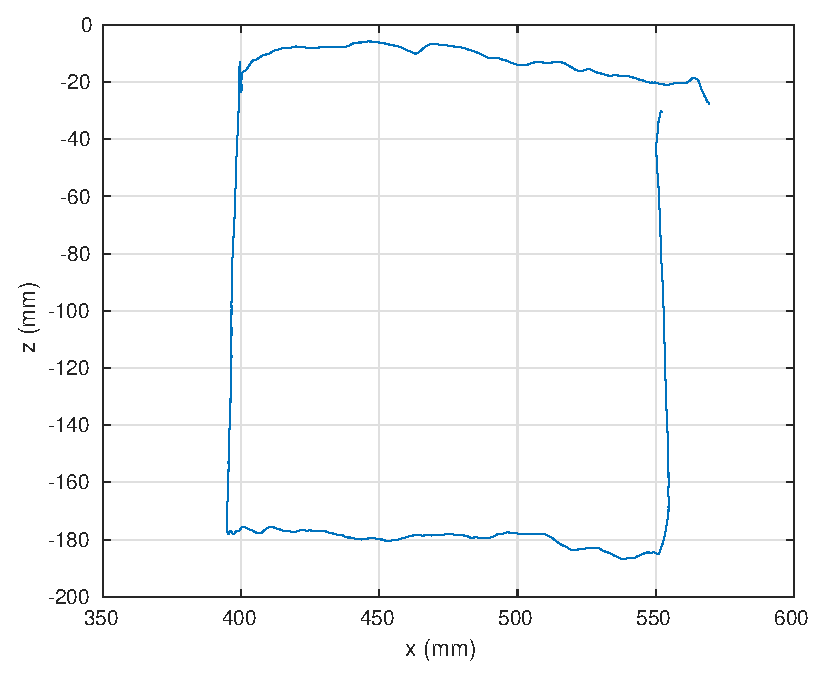
\includegraphics[width=0.5\linewidth]{./img/float2/xz.eps}
\caption{Plano x-z}
\end{figure}%\href{run:traject1.mp4}{
\begin{center}
\href{run:forca.mp4}{\textbf{Video}}% 
\end{center}
\end{frame}

\begin{frame}
\frametitle{Resultados experimentais - Controle de Força Approach}
\textbf{Resultados experimentais do controle de força na direção de approach com controlador PI de $k_p = 2$ e $k_i = 0.05$. }
\begin{figure}[H]
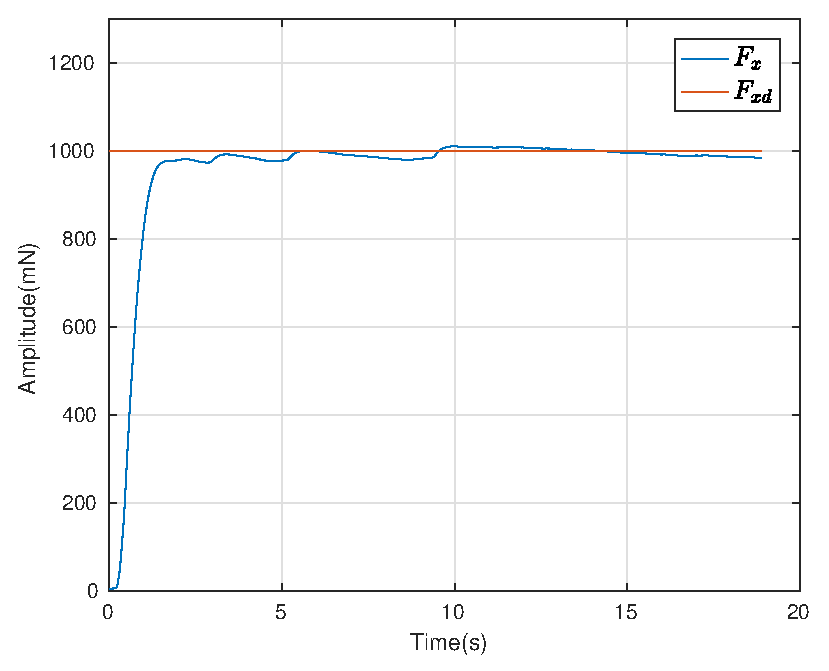
\includegraphics[width=0.5\linewidth]{./img/force1000_kp2_ki005/Fx.eps}
\end{figure}%\href{run:traject1.mp4}{
\begin{center}
\end{center}
\end{frame}

\begin{frame}
\frametitle{Resultados experimentais - Controle por Servo Visão}
\begin{figure}[H]
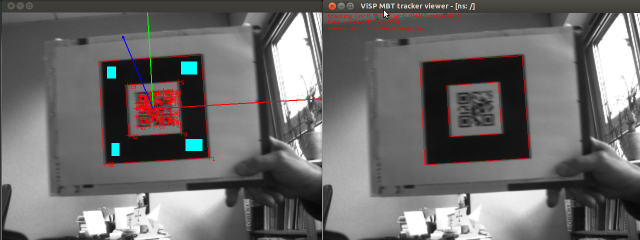
\includegraphics[width=0.5\linewidth]{./img/tracker_viewer-small.png}
\end{figure}%\href{run:traject1.mp4}{
\end{frame}

\begin{frame}
\frametitle{Conclusão}
\begin{itemize}
\item Resultados 
\item Controle Cinemático.
\item Sistemas de controle utilizando ROS.
\end{itemize}
\end{frame}


\begin{frame}
\Huge{\centerline{The End}}
\end{frame}

%----------------------------------------------------------------------------------------

\end{document} 